\documentclass[../main.tex]{subfiles}
\begin{document}

\ifSubfilesClassLoaded{
	\mainmatter
	\setcounter{chapter}{4}
}{}

\chapter{Analysis}
\label{ch:analysis}

\section{Data Sets}
SeaQuest received its first proton in the beginning of 2012, and began beam
commissioning. After a short commissioning run, the Main Injector was shut down for
upgrade. After the Main Injector restarted in 2013, the data collection began in
2014. The timeline and some important dates are tabulated in \cref{tab:dataset}.
\begin{table}[h!]
	\centering
	\begin{tabular}{ c c c }
		\hline
		Run & Experimental Conditions & Dates                    \\
		\hline
		2   & Roadset 57              & 06/25/2014 to 08/20/2014 \\
		    & Roadset 59              & 08/20/2014 to 09/03/2014 \\
		\hline
		N/A & D3p and D3m moved       & 10//03/2014              \\
		\hline
		3   & Roadset 62              & 11/08/2014 to 01/14/2015 \\
		    & Deuterium Change        & 11/13/2014               \\
		    & Deuterium Change        & 12/02/2014               \\
		    & Magnet Polarity flipped & 01/14/2015               \\
		    & Roadset 67              & 01/25/2015 to 06/19/2015 \\
		    & Deuterium Change        & 04/24/2014               \\
		    & D1 and H1 moved         & 05/13/2015               \\
		    & Roadset 70              & 06/19/2015 to 07/03/2015 \\
		\hline
		4   & Constant adjustments    & 11/13/2015 to 03/06/2016 \\
		5   & Roadset 78              & 03/06/2016 to 07/29/2016 \\
		6   & DAQ upgrade             & 01/14/2017 to 07/07/2017 \\ \hline
	\end{tabular}
	\caption{SeaQuest data sets and apparatus adjustments}
	\label{tab:dataset}
\end{table}

\section{Monte Carlo}
\label{sec:MC}
SeaQuest utilizes a GEANT4~\cite{agostinelli2003,allison2006,allison2016}
based Monte Carlo simulation (GMC) to simulate the
performance of the spectrometer and the acceptance. The GMC is based on the
E866 FastMC, a fortran-based simulation code, and is ported to SeaQuest and
modified according to SeaQuest's experimental configurations~\cite{kerns2018,prasad2020}.

\subsection{Dimuon generation}
As SeaQuest is mostly interested in dimuons with high mass and $x_F$, where the cross section
falls off rapidly, it is important to accurately determine the acceptance in this region.
If the generated dimuon distribution in GMC follows the expected cross section, most of the
generated events would be at the low mass and low $x_F$ region, where the cross section is large.
To ensure sufficient statistics across the full phase space of interested, the generated dimuon
distribution is uniform in both mass and $x_F$. The events are then weighted by the cross
section. This approach ensures high statistical precision in determining the acceptance
at high mass and $x_F$, while also preserving the expected dimuon kinematic distribution.

For a Drell-Yan dimuon, a mass and $x_F$ pair is chosen, the transverse momentum is also chosen.
For the $J/\psi$ and $\psi'$ dimuons, the dimuon mass is fixed at the mass of the corresponding
resonance.
Because the transverse momentum distribution ($p_T$) cannot be calculated using
fixed-order pQCD, it is typically parameterized using some functional form.
In the GMC simulation, the input $p_T$ distribution is based on the
Kaplan functional form~\cite{kaplan1978}.
\begin{equation}
	f\left(P_T^2\right) \propto \left(1+ P_T^2/p_1^2\right)^{-6},
	\label{eq:kaplan}
\end{equation}
The parameter $p_1$ controls the broadness of the $P_T$ distribution, and is
related to the average $P_T$ as follows
\begin{equation}
	\begin{split}
		\expval{P_T}   & = \frac{35\pi p_1}{256}, \\
		\expval{P_T^2} & = \frac{p_1^2}{4}.
		\label{eq:kaplan_mean}
	\end{split}
\end{equation}
The parameter $p_1$ is chosen to be \SI{2.8}{\GeV} for Drell-Yan and \SI{3}{\GeV} for charmonium
decays. These values are inherited from the previous \SI{800}{\GeV} Drell-Yan experiment at Fermilab.
It was later determined that these values of $p_1$ are not suitable for SeaQuest due the the lower
beam energy of \SI{120}{\GeV}, and the $P_T$ distribution is adjusted following a re-weighting procedure, which
would be described in \cref{subsec:pt_reweight}.

The dimuon angular distribution is typically calculated in the dimuon rest frame, known as
Collins-Soper frame~\cite{collins1977} and shown in \cref{fig:cs_frame}.
For the Drell-Yan events, the polar angle $\theta$ for the $\mu^-$ follows
a $1+\cos^2\theta$ distribution with a uniform azimuthal angular distribution $\phi$ in the Collins-Soper frame.
On the other hand, the angular distribution for the $J/\psi$ and $\psi'$ are uniform in
both $\theta$ and $\phi$.

\subsubsection{Transformation from Collins-Soper frame to Laboratory frame}
\begin{figure}[h!]
	\centering
	%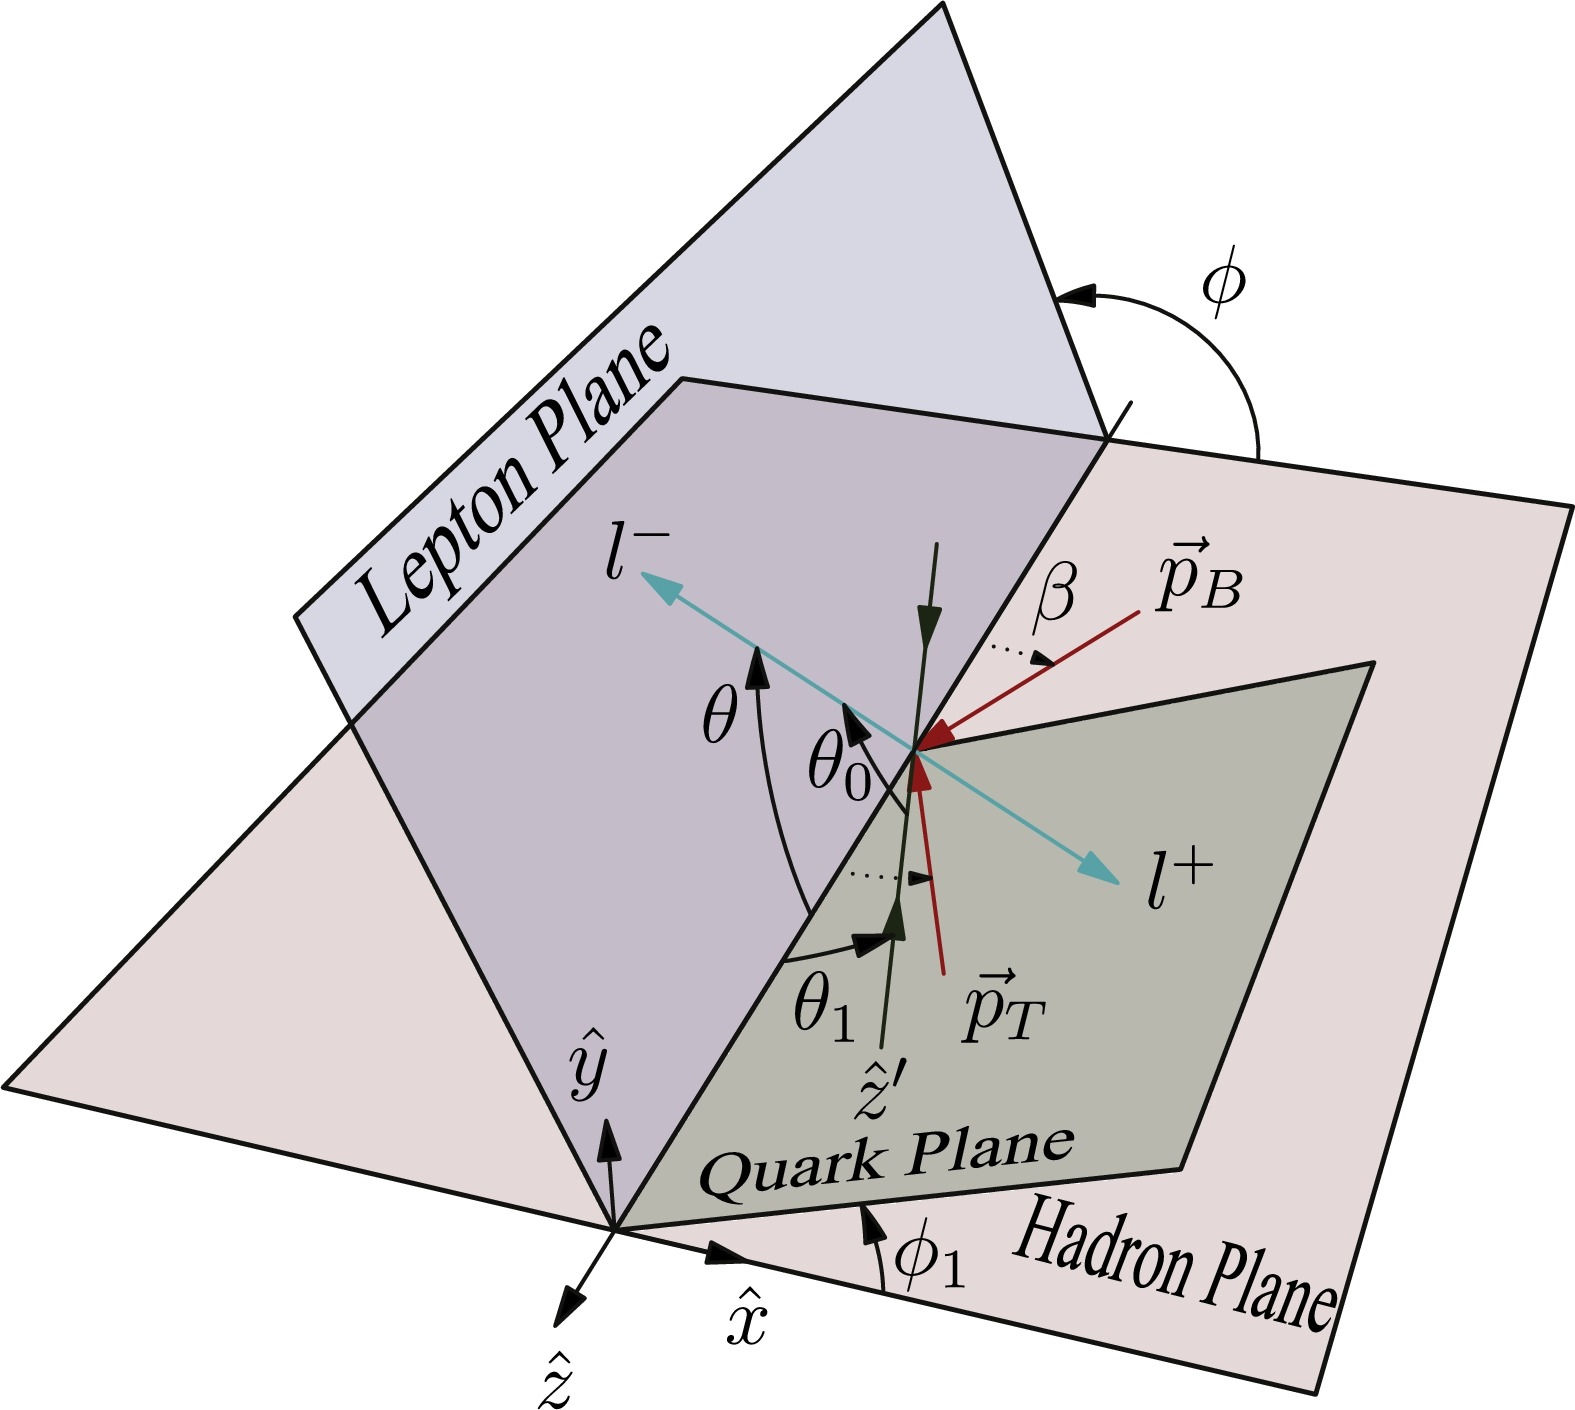
\includegraphics[width=0.6\linewidth]{Collins_Soper_frame}
	

\tikzset{every picture/.style={line width=0.75pt}} %set default line width to 0.75pt        

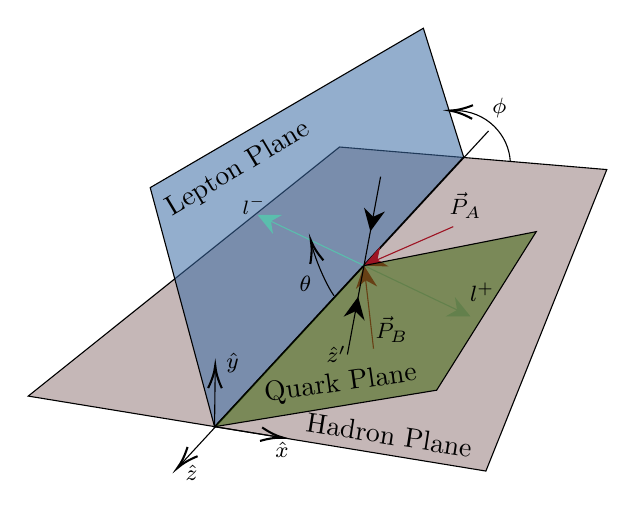
\begin{tikzpicture}[x=0.75pt,y=0.75pt,yscale=-1,xscale=1]
%uncomment if require: \path (0,300); %set diagram left start at 0, and has height of 300

%Straight Lines [id:da9360270151188433] 
\draw [color={rgb, 255:red, 90; green, 190; blue, 173 }  ,draw opacity=1 ]   (380.55,150.49) -- (332,127.36) ;
\draw [shift={(383.26,151.78)}, rotate = 205.47] [fill={rgb, 255:red, 90; green, 190; blue, 173 }  ,fill opacity=1 ][line width=0.08]  [draw opacity=0] (10.72,-5.15) -- (0,0) -- (10.72,5.15) -- (7.12,0) -- cycle    ;
%Shape: Polygon [id:ds3246920650393613] 
\draw  [fill={rgb, 255:red, 173; green, 152; blue, 152 }  ,fill opacity=0.7 ] (448.98,81.1) -- (390.73,226.35) -- (170.23,190.23) -- (238.46,135.64) -- (320.22,70.23) -- cycle ;
%Shape: Polygon [id:ds8122410861225874] 
\draw  [color={rgb, 255:red, 0; green, 0; blue, 0 }  ,draw opacity=1 ][fill={rgb, 255:red, 59; green, 107; blue, 164 }  ,fill opacity=0.55 ] (360.6,13) -- (229,89.8) -- (260,205) -- (380,75) -- cycle ;
%Straight Lines [id:da1607044272265945] 
\draw    (392,62.5) -- (243.36,223.53) ;
\draw [shift={(242,225)}, rotate = 312.71] [color={rgb, 255:red, 0; green, 0; blue, 0 }  ][line width=0.75]    (10.93,-3.29) .. controls (6.95,-1.4) and (3.31,-0.3) .. (0,0) .. controls (3.31,0.3) and (6.95,1.4) .. (10.93,3.29)   ;
%Straight Lines [id:da192804704893637] 
\draw [color={rgb, 255:red, 157; green, 20; blue, 36 }  ,draw opacity=1 ]   (375,108.6) -- (334.75,126.16) ;
\draw [shift={(332,127.36)}, rotate = 336.43] [fill={rgb, 255:red, 157; green, 20; blue, 36 }  ,fill opacity=1 ][line width=0.08]  [draw opacity=0] (10.72,-5.15) -- (0,0) -- (10.72,5.15) -- (7.12,0) -- cycle    ;
%Straight Lines [id:da9707379686817308] 
\draw [color={rgb, 255:red, 157; green, 20; blue, 36 }  ,draw opacity=1 ]   (336.6,167.4) -- (332.34,130.34) ;
\draw [shift={(332,127.36)}, rotate = 83.45] [fill={rgb, 255:red, 157; green, 20; blue, 36 }  ,fill opacity=1 ][line width=0.08]  [draw opacity=0] (10.72,-5.15) -- (0,0) -- (10.72,5.15) -- (7.12,0) -- cycle    ;
%Straight Lines [id:da6271845903433381] 
\draw [color={rgb, 255:red, 90; green, 190; blue, 173 }  ,draw opacity=1 ]   (332,127.36) -- (283.45,104.23) ;
\draw [shift={(280.74,102.94)}, rotate = 25.47] [fill={rgb, 255:red, 90; green, 190; blue, 173 }  ,fill opacity=1 ][line width=0.08]  [draw opacity=0] (10.72,-5.15) -- (0,0) -- (10.72,5.15) -- (7.12,0) -- cycle    ;
%Curve Lines [id:da8650973959260518] 
\draw    (317.57,141.86) .. controls (315.17,138.92) and (308.97,126.37) .. (306.77,117.04) ;
\draw [shift={(306.37,115.15)}, rotate = 74.54] [color={rgb, 255:red, 0; green, 0; blue, 0 }  ][line width=0.75]    (10.93,-3.29) .. controls (6.95,-1.4) and (3.31,-0.3) .. (0,0) .. controls (3.31,0.3) and (6.95,1.4) .. (10.93,3.29)   ;
%Straight Lines [id:da8376735939956365] 
\draw    (260,205) -- (291.25,210.02) ;
\draw [shift={(293.22,210.33)}, rotate = 189.12] [color={rgb, 255:red, 0; green, 0; blue, 0 }  ][line width=0.75]    (10.93,-3.29) .. controls (6.95,-1.4) and (3.31,-0.3) .. (0,0) .. controls (3.31,0.3) and (6.95,1.4) .. (10.93,3.29)   ;
%Straight Lines [id:da23422313993045396] 
\draw    (260,205) -- (260.31,177.44) ;
\draw [shift={(260.33,175.44)}, rotate = 90.65] [color={rgb, 255:red, 0; green, 0; blue, 0 }  ][line width=0.75]    (10.93,-3.29) .. controls (6.95,-1.4) and (3.31,-0.3) .. (0,0) .. controls (3.31,0.3) and (6.95,1.4) .. (10.93,3.29)   ;
%Straight Lines [id:da6033196978161374] 
\draw    (340,84.52) -- (332,127.36) ;
\draw [shift={(335.08,110.86)}, rotate = 280.58] [fill={rgb, 255:red, 0; green, 0; blue, 0 }  ][line width=0.08]  [draw opacity=0] (10.72,-5.15) -- (0,0) -- (10.72,5.15) -- (7.12,0) -- cycle    ;
%Shape: Polygon [id:ds8570377916667694] 
\draw  [fill={rgb, 255:red, 60; green, 101; blue, 10 }  ,fill opacity=0.55 ] (415,111) -- (367,187.4) -- (260,205) -- (332,127.36) -- cycle ;
%Straight Lines [id:da24422947787646188] 
\draw    (332,127.36) -- (324,170.19) ;
\draw [shift={(329.19,142.38)}, rotate = 100.58] [fill={rgb, 255:red, 0; green, 0; blue, 0 }  ][line width=0.08]  [draw opacity=0] (10.72,-5.15) -- (0,0) -- (10.72,5.15) -- (7.12,0) -- cycle    ;
%Curve Lines [id:da6714496890784999] 
\draw [color={rgb, 255:red, 0; green, 0; blue, 0 }  ,draw opacity=1 ]   (402.47,77.08) .. controls (401.79,64.74) and (391.36,52.48) .. (375.17,52.63) ;
\draw [shift={(373.38,52.69)}, rotate = 3.59] [color={rgb, 255:red, 0; green, 0; blue, 0 }  ,draw opacity=1 ][line width=0.75]    (10.93,-3.29) .. controls (6.95,-1.4) and (3.31,-0.3) .. (0,0) .. controls (3.31,0.3) and (6.95,1.4) .. (10.93,3.29)   ;

% Text Node
\draw (392.6,45.56) node [anchor=north west][inner sep=0.75pt]  [font=\fontsize{0.82em}{0.99em}\selectfont]  {$\phi $};
% Text Node
\draw (299.71,131.28) node [anchor=north west][inner sep=0.75pt]  [font=\fontsize{0.82em}{0.99em}\selectfont]  {$\theta $};
% Text Node
\draw (272.09,92.84) node [anchor=north west][inner sep=0.75pt]  [font=\fontsize{0.71em}{0.85em}\selectfont]  {$l^{-}$};
% Text Node
\draw (381.89,134.34) node [anchor=north west][inner sep=0.75pt]  [font=\fontsize{0.82em}{0.99em}\selectfont]  {$l^{+}$};
% Text Node
\draw (288.09,211.04) node [anchor=north west][inner sep=0.75pt]  [font=\fontsize{0.82em}{0.99em}\selectfont]  {$\hat{x}$};
% Text Node
\draw (244.76,222.38) node [anchor=north west][inner sep=0.75pt]  [font=\fontsize{0.82em}{0.99em}\selectfont]  {$\hat{z}$};
% Text Node
\draw (264.42,168.49) node [anchor=north west][inner sep=0.75pt]  [font=\fontsize{0.82em}{0.99em}\selectfont]  {$\hat{y}$};
% Text Node
\draw (232.9,95.34) node [anchor=north west][inner sep=0.75pt]  [font=\normalsize,rotate=-329.15] [align=left] {Lepton Plane};
% Text Node
\draw (281.87,182.79) node [anchor=north west][inner sep=0.75pt]  [font=\normalsize,rotate=-351.89] [align=left] {Quark Plane};
% Text Node
\draw (304.02,196.65) node [anchor=north west][inner sep=0.75pt]  [font=\normalsize,rotate=-9.03] [align=left] {Hadron Plane};
% Text Node
\draw (312.76,164.73) node [anchor=north west][inner sep=0.75pt]  [font=\fontsize{0.82em}{0.99em}\selectfont]  {$\hat{z} '$};
% Text Node
\draw (372.05,91.11) node [anchor=north west][inner sep=0.75pt]  [font=\fontsize{0.82em}{0.99em}\selectfont]  {$\vec{P}_{A}$};
% Text Node
\draw (336.3,150.78) node [anchor=north west][inner sep=0.75pt]  [font=\fontsize{0.82em}{0.99em}\selectfont]  {$\vec{P}_{B}$};


\end{tikzpicture}


	\caption{Definition of the Collins–Soper frame and various angles and planes in the rest frame of the dimuon.
		The hadron plane is formed by $\vec{P}_A$ and $\vec{P}_B$, the momentum vectors of the colliding hadrons.
		The $\hat{x}$ and $\hat{z}$ axes both lie on the hadron plane, with $\hat{z}$ bisecting $\vec{P}_A$ And
		$\vec{P}_B$. Adapted from Ref.~\cite{peng2019}}
	\label{fig:cs_frame}
\end{figure}
The Collins-Soper frame is defined in the rest frame of the dimuon.
The hadron plane is formed by the momentum vectors of the two interacting hadrons
($\vec{P}_A$ and $\vec{P}_B$). The $\hat{x}$ and $\hat{z}$ axes are chosen to be on the hadron plane.
The Collins-Soper frame is defined such that the $\hat{z}$ axis bisecting the $\vec{P}_A$ and $-\vec{P}_B$
vectors and $\hat{x}$ is along the dilepton transverse momentum. 
The outgoing leptons $l^+$ and $l^-$ are emitted back-to-back, forming the lepton plane, 
with polar angle $\theta$ and azimuthal angle $\phi$ for $l^-$.
The annihilating quark and antiquark annihilate collinearly with equal momenta along $\hat{z}'$.
The quark momentum vector $\hat{z}'$ and $\hat{z}$ axis forms the quark plane, which can be offset from the
hadron plane.

To transform from the Collins-Soper frame to lab frame, three Lorentz transforms are applied.
The first transformation boosts along the virtual photon's $-P_T$ direction, a second transformation then
boosts along the $-z$ direction to reach the hadron-hadron center of mass frame. A final transformation
then boosts along the $-z$ direction to reach the lab frame~\cite{Don-1926}.

The first transform from the Collins-Soper frame is along the $\hat{x}$ direction (or along the dilepton $-p_T$).
The $\gamma$ and $\beta$ for this boost are given as
\begin{equation}
	\begin{split}
		\gamma_1 & = \frac{\sqrt{p_T^2 + M^2}}{M},\\
		\beta_1 & = \frac{M}{\sqrt{p_T^2 + M^2}}.
	\end{split}
\end{equation}
The $x$-$y$ axes are then rotated along $z$ direction by $\phi_\gamma$, as the dilepton $P_T$
does not necessarily lie on the $x$-axis in the lab frame.
This angle $\phi_\gamma$ is randomly selected from a uniform distribution.

The next transform is along the $z$-axis to reach the hadron-hadron center of mass frame.
\begin{equation}
	\begin{split}
		\gamma_2 &= \frac{\sqrt{P_L^2 + M^2}}{M},\\
		\beta_2 & = \frac{M}{\sqrt{p_L^2 + M^2}},
	\end{split}
\end{equation}
where $P_L$ and $M$ are the longitudinal momentum and mass of the virtual photon respectively.
The final transform along the $z$-axis to the lab frame is given by
\begin{equation}
	\begin{split}
		\gamma_3 &= \frac{E_{\mathrm{beam}}+m_{\mathrm{proton}}}{\sqrt{s}},\\
		\beta_3 & = \frac{P_{\mathrm{proton}}}{E_{\mathrm{beam}}+m_{\mathrm{proton}}}.
	\end{split}
\end{equation}

\subsubsection{Cross section weighting}
To recover the expected kinematics distributions, 
each event is assigned a weight based on the cross section.
The Drell-Yan cross section is calculated based on the kinematics of the generated events. 
The leading order cross section is calculated with the CT14 pdf.
The NLO effect is then included using 2-dimensional K-Factor~\cite{shivangi-1747}, which
is defined as the ratio of the NLO cross section over LO cross section and is
calculated using DYNNLO (see \cref{sec:DYNNLO}).
The proton on deuterium cross section is calculated using the charge symmetry.
Assuming negligible nuclear correction, the proton on deuterium cross section are calculated
as the sum of $p+p$ and $p+n$ cross section.

The cross section for the $J/\psi$ is parameterized by a Gaussian in $x_F$ and fitted to the
calculation using color evaporation model, with the normalization taken from a particularization by E789~\cite{schub1995}.
\begin{equation}
	\dv{\sigma_{J/\psi}}{x_F} = Ae^{-B\sqrt{\tau}} \left[ \frac{e^{-x^2_F/2C^2}}{\sqrt{2\pi}C} \right],
\end{equation}
where $A=\SI{1464}{\nano\barn}$, $B=16.66$, $C=0.2398$, and $\tau=m^2_{J/\psi}/s$.
The branching ration $B\left(J/\psi\rightarrow \mu^+ \mu^-\right)=0.0594$ is also included.
The $\psi'$ cross section is based to $J/\psi$ cross section, with an additional factor
$\left[B\left(\psi'\rightarrow \mu^+ \mu^-\right)\cross\sigma_{\psi'}\right]/\left[B\left(J/\psi\rightarrow \mu^+ \mu^-\right)\cross\sigma_{J/\psi}\right]=0.019$.

\subsection{Messy and Clean Monte Carlo}
\label{subsec:messyMC}
Before reconstruction, the resolution and efficiency of the detectors needs to be included.
This step is known as realization.
From previous studies, the efficiency for the chambers is determined to be \SI{\sim 94}{\percent}
with a resolution of \SI{\sim 0.04}{\cm}. Therefore for all chamber hits, \SI{6}{\percent} of
hits are dropped randomly, with a Gaussian smearing applied to the drift distance for the remaining
hits with a width of \SI{0.04}{\cm}. The Monte Carlo data are now ready for track reconstruction and analysis.
This is labeled as ``clean Monte Carlo'', and is used in acceptance studies without the
rate dependent effects.

If we are interested in the rate dependent effects, there is an option to embed NIM-3 hits into
the clean Monte Carlo to create what is known as ``messy Monte Carlo''.
The purpose is to simulate the noise and background hits in the spectrometer. By including noise
and background hit, we can understand the performance of our reconstruction software at different
occupancy.
Since the NIM-3 trigger randomly, the hit distribution in each detector would be reflect
the background and noise hits caused by the beam. However, as the probability of a dimuon event
is higher at higher beam intensity, the signal (MATRIX-1) events would have a significantly higher
average occupancy than the NIM-3 events, as shown in \cref{fig:NIM3_FPGA1}.
The input occupancy distribution should have little or no
effect on the reconstruction efficiency, as we are only interested the fraction of events that was
successfully reconstructed in each occupancy bin, not the absolute number of events in each bin.
However, the occupancy profile could have significant effect when using the occupancy integrated
messy Monte Carlo such as mass fit studies. Therefore, when sampling the NIM-3 events, the occupancy ratio
of the MATRIX-1 and NIM-3 events is used as weights, and high occupancy NIM-3 would have a higher
probability to be used, where as only a small fraction of lower occupancy NIM-3 events would be used.

\begin{figure}[h!]
	\centering
	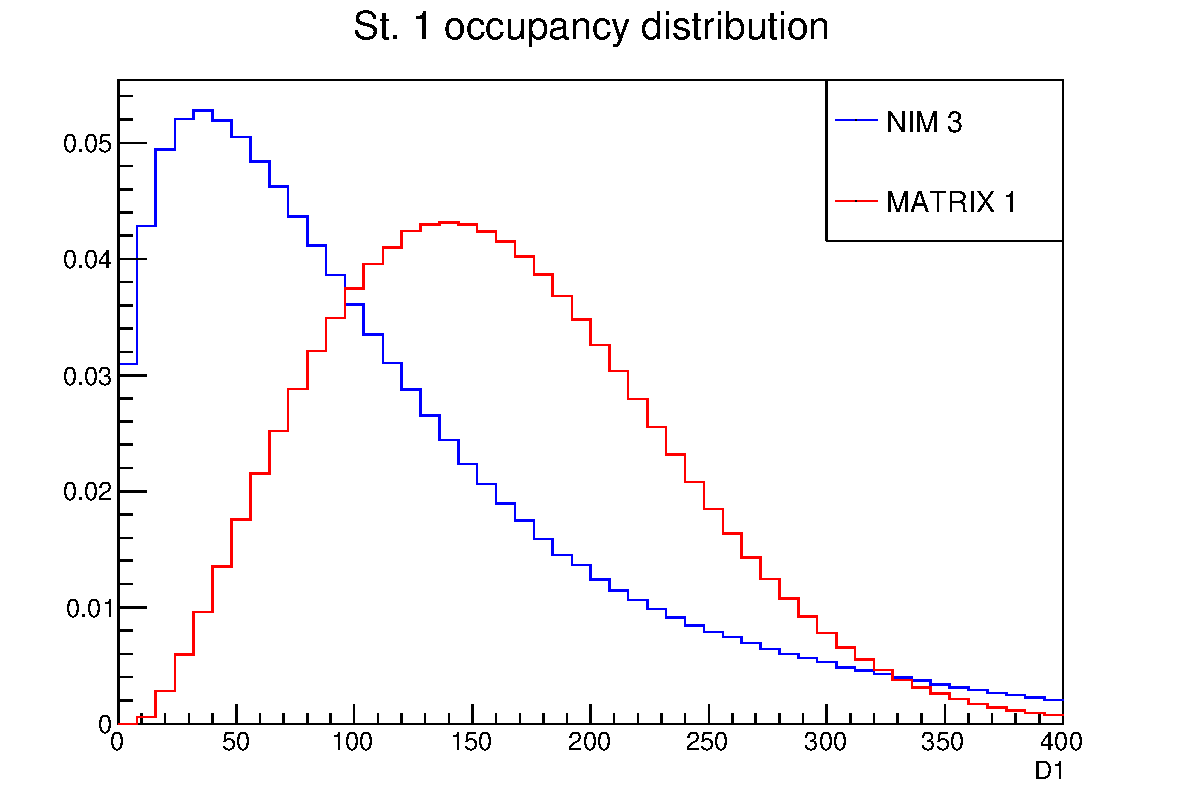
\includegraphics[width=0.6\linewidth]{rs67_NIM3_FPGA1}
	\caption{The St.~1 occupancy distribution for MATRIX-1 and NIM-3 events. Both histograms are normalized
		to unit area. The average occupancy for the MATRIX-1 events are higher as the probability of observing
		a dimuon is higher at higher beam intensity, and the beam intensity is strongly related to the chamber
		occupancy.
	}
	\label{fig:NIM3_FPGA1}
\end{figure}

\subsection{Maximum dimuon \texorpdfstring{$P_T$}{P\_T}}
\label{subsec:max_pt}
One of the changes I made to the Monte Carlo generator during this study
is the maximum transverse momentum of the virtual photon.

Let $\mathbf{P}_\gamma$ and $\mathbf{P}_R$ be the four momenta of the virtual photon and residual system respectively.
In the hadron-hadron center-of-mass frame, 
\begin{equation}
	\begin{split}
		\mathbf{P}_\gamma &= \begin{bmatrix}
			E_\gamma & \vec{P}
		\end{bmatrix},	\\
		\mathbf{P}_R &= \begin{bmatrix}
			E_R & -\vec{P}
		\end{bmatrix},
	\end{split}
\end{equation}
and 
\begin{equation}
    \begin{split}
        E^2_R &= M_R^2 + P^2,\\
        E^2_\gamma &= M_\gamma^2 + P^2,
    \end{split}
\end{equation}
where $M_\gamma$ and $M_R$ are the mass of the virtual photon and residual system respectively.
From the conservation of energy, the sum of virtual photon and residual system momenta should
equal the center of mass energy $\sqrt{s}$.
\begin{equation}
	\begin{split}
		s &=\left( \mathbf{P_R}+\mathbf{P_\gamma} \right)^2 = \left(E_R+E_\gamma\right)^2\\
		&= E_R^2+E_\gamma^2+2E_R E_\gamma.\\
	\end{split}
\end{equation}
Therefore the magnitude of the virtual photon momentum $\vec{P}$ is given by
\begin{equation}
	P^2 = \frac{1}{4s} \left[ s^2 + \left(M_R^2 - M_\gamma^2\right)^2 -2s\left(M^2_R+M_\gamma^2\right) \right]
\end{equation}

For maximum $P$, the mass of the residual system should be approaching zero. Therefore,
\begin{equation}
    \begin{split}
        \left(P^{\mathrm{max}}\right)^2 &= \frac{1}{4s} \left[ s^2 +  M_\gamma^4 -2sM_\gamma^2\right]\\
        &=\frac{s}{4}\left[ 1 -M_\gamma^2/s\right]^2.\\
    \end{split}
\end{equation}

The virtual photon momentum, $\vec{P}$, can be decompose into the longitudinal ($P_L$) and transverse ($P_T$)
components. The maximum $P_L$ is achieved when $P_T$ is approaching zero. Hence
\begin{equation}
	P_L^{\mathrm{max}} = \frac{\sqrt{s}}{2}\left(1-\frac{M_\gamma^2}{s}\right).
\end{equation}
Therefore, we define Feynman $x$ as
\begin{equation}
	x_F = \frac{P_L}{P_L^{\mathrm{max}}}=\frac{2P_L}{\sqrt{s}\left(1-M_\gamma^2/2\right)}.
\end{equation}
For a fixed $x_F$, the maximum $P_T$ carried by the virtual photon
is given by
\begin{equation}
	\left(P_T^{\mathrm{max}}\right)^2 = \frac{s}{4} \left[1-M^2_\gamma/s\right]^2\left[1-x_F^2\right].
	\label{eq:pTmax}
\end{equation}

Earlier versions of the SeaQuest Monte Carlo generators used an inconsistent definition of $x_F$
and $P_T^{\mathrm{max}}$, resulting in an incomplete coverage of the kinematic phase space.

\subsection{\texorpdfstring{$P_T$}{P\_T} re-weighting in Monte Carlo}
\label{subsec:pt_reweight}
This was first studied by S.~Prasad~\cite{prasad2020}.
In the GMC, the transverse momentum distribution randomly follows the Kaplan functional form
\cref{eq:kaplan},
with $p_1$ is set to \SI{2.8}{\GeV} for Drell-Yan and \SI{3}{\GeV} for charmonium
decays. If the chosen $P_T$ exceeds $P_T^{\mathrm{max}}$ in \cref{eq:pTmax}
and does not satisfy the kinematic constraint, a new $P_T$ will be chosen until
the constraint is satisfied.

The chosen value of $p_1$ is taken from experiments conducted at higher
energies, and may not be suitable to the SeaQuest kinematic. An additional weight is
applied to account for the difference between the $P_T$ distribution in the MC input
and in the real data. In addition, the $P_T$ distribution can also depend on $x_F$.
The $x_F$ dependence of the $P_T$ distribution has been reported in the pion induced
Drell-Yan experiment E615~\cite{conway1989}. The $x_F$ and $\sqrt{s}$ dependence in
proton induced Drell-Yan has also been reported in Ref.~\cite{prasad2020}.

In this analysis, a different re-weighting formula is used. Because of the way $P_T$ is chosen
in the event generator, the probability density function is normalized to unity as follows
\begin{equation}
	\int^{\left(P_T^{\mathrm{max}}\right)^2}_0 dP_T^2 \frac{N}{\left(1+ P_T^2/p_1^2\right)^6}=1
\end{equation}
where $N$ is the normalization constant and is given by
\begin{equation}
	N=\frac{5}{p_1^2-p_1^2\left[ 1+ \left(P_T^{\mathrm{max}}\right)^2/p_1^2\right]^{-5}}.
\end{equation}
Therefore the $p_T$ reweight is given by
\begin{equation}
	P_T \mathrm{ reweight}\left(m,x_F\right)=
	\frac{\left(1 + \frac{p_T^2}{2.8^2} \right)^6}{\left(1 + \frac{p_T^2}{\left(p_1\left(x_F\right)\right)^2} \right)^6} \frac{2.8^2}{\left(p_1\left(x_F\right)\right)^2}\frac{1-\left[ 1+ \frac{\left(P_T^{\mathrm{max}}\left(m,x_F\right)\right)^2}{2.8^2}\right]^{-5}}{1-\left[ 1+ \frac{\left(P_T^{\mathrm{max}}\left(m,x_F\right)\right)^2}{\left(p_1\left(x_F\right)\right)^2}\right]^{-5}}.
	\label{eq:pT_reWeight}
\end{equation}
The addition of the last factor in \cref{eq:pT_reWeight}, as compared to previous studies,
is to ensure the normalization is preserved and would not affect the other kinematic
distributions at generator level.

While we could modify the input $P_T$ distribution in the Monte Carlo event generator,
it is decided to utilize this re-weighting procedure as this would allow for
more iterations of refinement with less computation overhead.

\section{Event Reconstruction}
The SeaQuest reconstruction is done using kTracker, primarily developed by K.~Liu~\cite{kTracker}.
One of my responsibility is the reconstruction of the run 5 and run 6 data. In order to reduce the processing
time, we utilize the Open Science Grid~\cite{pordes2007,sfiligoi2009,osg2006} to run multiple kTracker
instances and process multiple events in parallel.
I have also utilized Apptainer (formerly known as Singularity)~\cite{kurtzer2021} to maintain better control of the
runtime environment.

The reconstruction is divided into three parts: EventReducer, kFastTracking, and kVertex.
EventReducer prepares all the events for reconstruction by removing extraneous hits that are
unlikely to be part of a valid track. This is done to speed up the reconstructions. Then, kFastTracking
will identify all valid tracks in the events. Finally, kVertex will try all possible track combinations
to identify valid dimuons and reconstruct the dimuon kinematics.

\subsection{Spill-level Cuts}
During the offline decoding process, several data quality cuts are applied.
These cut are to ensure the data taking conditions were both normal and accurately recorded.
During analysis, this is typically done by querying the database
and requiring the data quality equals to zero in the spill table.
These cuts are tabulated in \cref{tab:spillQA}.
\begin{table}[h!]
	\centering
	\caption{Spill-level cuts for the different run period}
	\label{tab:spillQA}
	\begin{tabular}{l|llll}
		\hline
		Description                                                                     & Roadset 57 \& 59 & Roadset 62, 67 \& 70 & Run 5          & Run 6          \\ \hline
		Duty Factor                                                                     & $[15,60] $       & $[10, 60] $          & $[10, 60] $    & $[10, 60] $    \\
		G2SEM                                                                           & $[2e12, 1e13]$   & $[2e12, 1e13]$       & $[2e12, 1e13]$ & $[2e12, 1e13]$ \\
		QIEsum                                                                          & $[4e10, 1e12]$   & $[4e10, 1e12]$       & $[4e10, 1e12]$ & $[4e10, 1e12]$ \\
		FMAG                                                                            & $[1950, 2050]$   & $[1950, 2050]$       & $[1950, 2050]$ & $[1950, 2050]$ \\
		KMAG                                                                            & $[1550,1650]$    & $[1550,1650]$        & $[1550,1650]$  & $[1550,1650]$  \\
		TargetPos                                                                       & $[1,7]$          & $[1,7]$              & $[1,7]$        & $[1,7]$        \\
		Inhibit                                                                         & $[4e9, 1e11]$    & $[4e9, 2e11]$        & $[4e9, 2e11]$  & $[4e9, 2e11]$  \\
		Busy                                                                            & $[4e9, 1e11]$    & $[4e9, 1e11]$        & $[4e9, 1e11]$  & $[4e9, 1e11]$  \\
		AcceptedFPGA1                                                                   & $[1e3, 8e3]$     & $[1e2, 6e3]$         & $[1e2, 6e3]$   & $[1e2, 6e3]$   \\
		AfterInhFPGA1                                                                   & $[1e3, 3e4]$     & $[1e2, 1e4]$         & $[1e2, 1e4]$   & $[1e2, 1e4]$   \\
		Accepted/AfterInh                                                               & $[0.2, 0.9]$     & $[0.2, 1.05]$        & $[0.2, 1.05]$  & $[0.2, 1.05]$  \\
		TSGo                                                                            & $[1e3, 8e3]$     & $[1e2, 6e3]$         & $[1e2, 6e3]$   & $[1e2, 6e3]$   \\
		\begin{tabular}[c]{@{}l@{}}\# of Tracks found \\ per AcceptedFPGA1\end{tabular} &                  &                      &                & $(0.4,1.6)$    \\ \hline
	\end{tabular}
\end{table}



\subsection{Pre-tracking Cuts}
In order to speed up the reconstruction, various types of chamber hits are removed, as
they are less likely to be part of a muon track. This is handled by the EventReducer.

\paragraph{In-time cut}
During data taking, the TDC time window is deliberately set to be larger than the in-time
window. This is done to avoid data loss in case of timing drift~\cite{daniel-4924}.
During the offline processing, only in-time hits will be kept. This cut is applied to
all detectors.

\paragraph{After-pulse cut}
Due to the tendency of the wire chamber channels to `ring' after being hit,
a single charge particle may produce multiple pulses on the same
wire in quick succession. Therefore, if there are multiple TDC hits on same chamber wire
within a small predefined time window, only the first hit will be kept.

\paragraph{Cluster removal cut}
There are three types of cluster hits: cell-edge hits, delta-rays and electronic noise.

When a muon passes through the wire plane near the cell edge, it will often cause two adjacent
wires to fire. If the drift distance of one hit is more than \SI{90}{\percent} of the cell width,
while the drift distance of the other hit is less than \SI{40}{\percent} of the cell width, the hit
with larger drift distance will be discarded.

Delta rays are electrons knocked off by the primary radiation particle when passing
through the chamber. The knocked off electron is capable of producing secondary ionization.
Some of these electrons scatter at large angles and travel parallel to the chamber plane
and fire several wire. Since the primary muon would locate on either side on the hit cluster,
only edge hits are retained.

The chamber electronics are also prone to electronic noise, thereby creating clusters of
hits that do not correspond to real particle. During the offline analysis, if a string of
3 or more hits on adjacent wires have similar TDC time, with average time difference between
hits less than \SI{10}{\ns}, all these hits are considered electronic noise and are removed.

\begin{figure}
	\centering
	

\tikzset{every picture/.style={line width=0.75pt}} %set default line width to 0.75pt        

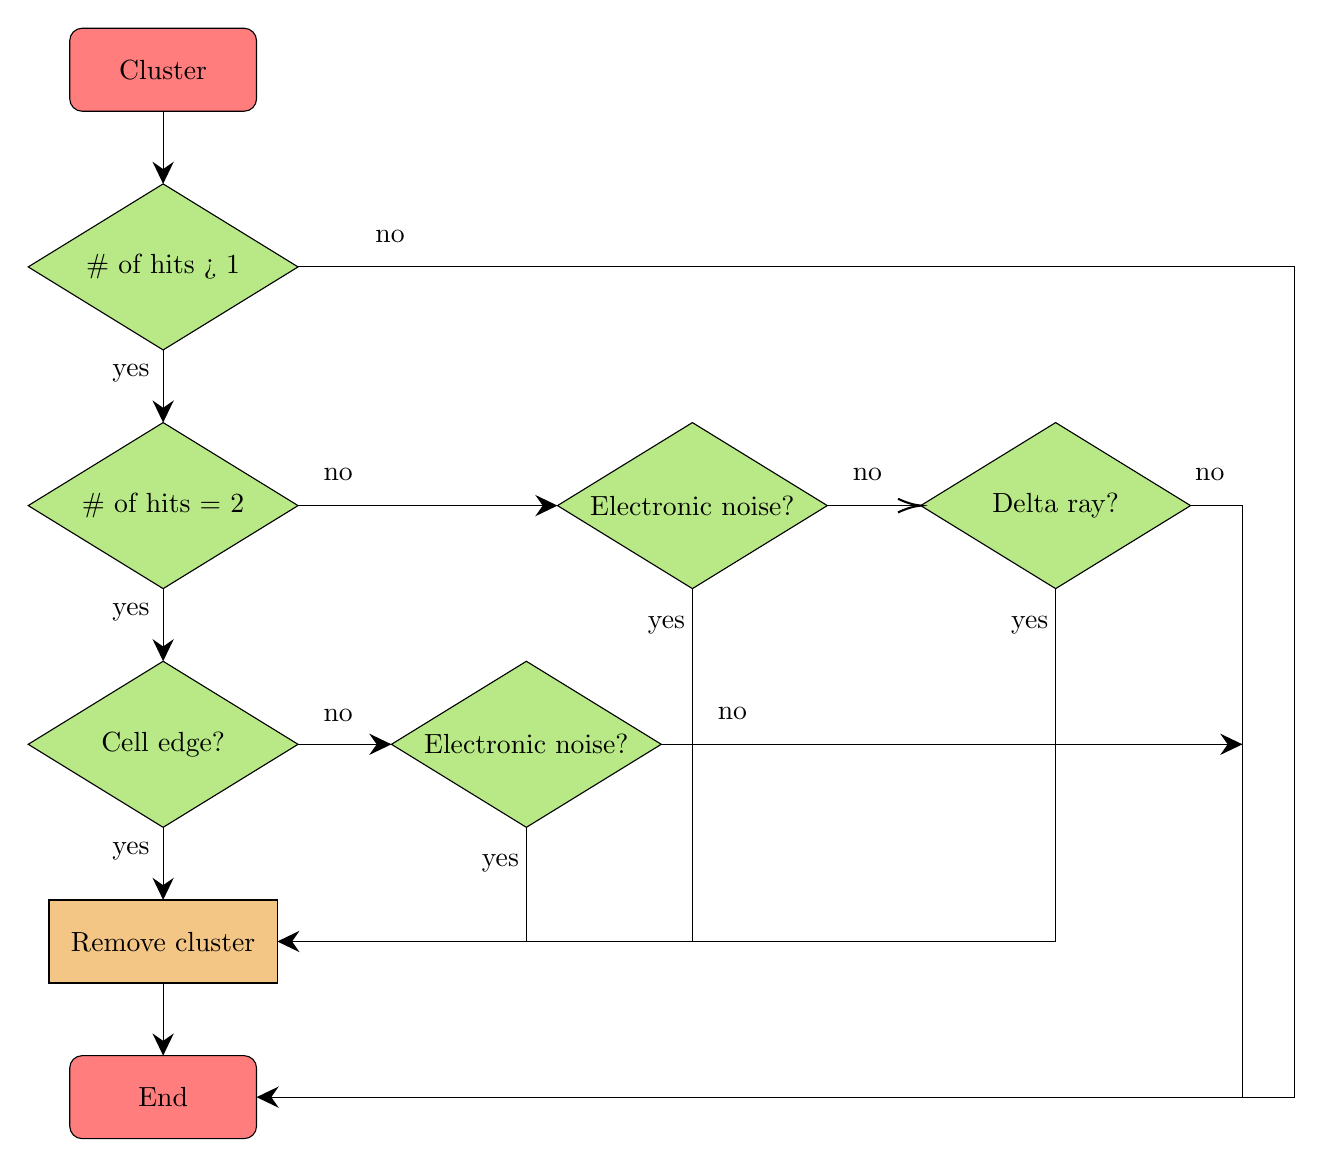
\begin{tikzpicture}[x=0.75pt,y=0.75pt,yscale=-1,xscale=1]
%uncomment if require: \path (0,549); %set diagram left start at 0, and has height of 549

%Rounded Rect [id:dp1662492856064861] 
\draw  [fill={rgb, 255:red, 255; green, 125; blue, 125 }  ,fill opacity=1 ] (20,11) .. controls (20,7.69) and (22.69,5) .. (26,5) -- (104,5) .. controls (107.31,5) and (110,7.69) .. (110,11) -- (110,39) .. controls (110,42.31) and (107.31,45) .. (104,45) -- (26,45) .. controls (22.69,45) and (20,42.31) .. (20,39) -- cycle ;
%Flowchart: Decision [id:dp816640900376574] 
\draw  [fill={rgb, 255:red, 184; green, 233; blue, 134 }  ,fill opacity=1 ] (240,310) -- (305,350) -- (240,390) -- (175,350) -- cycle ;
%Flowchart: Decision [id:dp3056798665151721] 
\draw  [fill={rgb, 255:red, 184; green, 233; blue, 134 }  ,fill opacity=1 ] (320,195) -- (385,235) -- (320,275) -- (255,235) -- cycle ;
%Straight Lines [id:da43332826362990795] 
\draw    (65,45) -- (65,77) ;
\draw [shift={(65,80)}, rotate = 270] [fill={rgb, 255:red, 0; green, 0; blue, 0 }  ][line width=0.08]  [draw opacity=0] (10.72,-5.15) -- (0,0) -- (10.72,5.15) -- (7.12,0) -- cycle    ;
%Straight Lines [id:da1721933893310973] 
\draw    (65,160) -- (65,192) ;
\draw [shift={(65,195)}, rotate = 270] [fill={rgb, 255:red, 0; green, 0; blue, 0 }  ][line width=0.08]  [draw opacity=0] (10.72,-5.15) -- (0,0) -- (10.72,5.15) -- (7.12,0) -- cycle    ;
%Straight Lines [id:da7629068372469668] 
\draw    (130,235) -- (252,235) ;
\draw [shift={(255,235)}, rotate = 180] [fill={rgb, 255:red, 0; green, 0; blue, 0 }  ][line width=0.08]  [draw opacity=0] (10.72,-5.15) -- (0,0) -- (10.72,5.15) -- (7.12,0) -- cycle    ;
%Straight Lines [id:da2682927683523839] 
\draw    (130,350) -- (172,350) ;
\draw [shift={(175,350)}, rotate = 180] [fill={rgb, 255:red, 0; green, 0; blue, 0 }  ][line width=0.08]  [draw opacity=0] (10.72,-5.15) -- (0,0) -- (10.72,5.15) -- (7.12,0) -- cycle    ;
%Shape: Rectangle [id:dp937184065620104] 
\draw  [fill={rgb, 255:red, 244; green, 198; blue, 133 }  ,fill opacity=1 ] (10,425) -- (120,425) -- (120,465) -- (10,465) -- cycle ;
%Straight Lines [id:da7703418793683412] 
\draw    (130,120) -- (610,120) -- (610,520) -- (113,520) ;
\draw [shift={(110,520)}, rotate = 360] [fill={rgb, 255:red, 0; green, 0; blue, 0 }  ][line width=0.08]  [draw opacity=0] (10.72,-5.15) -- (0,0) -- (10.72,5.15) -- (7.12,0) -- cycle    ;
%Straight Lines [id:da9159913508501855] 
\draw    (560,235) -- (585,235) -- (585,520) ;
%Straight Lines [id:da9876271822829807] 
\draw    (305,350) -- (582,350) ;
\draw [shift={(585,350)}, rotate = 180] [fill={rgb, 255:red, 0; green, 0; blue, 0 }  ][line width=0.08]  [draw opacity=0] (10.72,-5.15) -- (0,0) -- (10.72,5.15) -- (7.12,0) -- cycle    ;
%Straight Lines [id:da06393806538831526] 
\draw    (320,275) -- (320,445) -- (123,445) ;
\draw [shift={(120,445)}, rotate = 360] [fill={rgb, 255:red, 0; green, 0; blue, 0 }  ][line width=0.08]  [draw opacity=0] (10.72,-5.15) -- (0,0) -- (10.72,5.15) -- (7.12,0) -- cycle    ;
%Straight Lines [id:da5394607907564043] 
\draw    (240,390) -- (240,445) ;
%Rounded Rect [id:dp009664062523304096] 
\draw  [fill={rgb, 255:red, 255; green, 125; blue, 125 }  ,fill opacity=1 ] (20,506) .. controls (20,502.69) and (22.69,500) .. (26,500) -- (104,500) .. controls (107.31,500) and (110,502.69) .. (110,506) -- (110,534) .. controls (110,537.31) and (107.31,540) .. (104,540) -- (26,540) .. controls (22.69,540) and (20,537.31) .. (20,534) -- cycle ;
%Flowchart: Decision [id:dp9024602763737721] 
\draw  [fill={rgb, 255:red, 184; green, 233; blue, 134 }  ,fill opacity=1 ] (65,80) -- (130,120) -- (65,160) -- (0,120) -- cycle ;
%Flowchart: Decision [id:dp13524885014891452] 
\draw  [fill={rgb, 255:red, 184; green, 233; blue, 134 }  ,fill opacity=1 ] (65,195) -- (130,235) -- (65,275) -- (0,235) -- cycle ;
%Flowchart: Decision [id:dp2973369440123841] 
\draw  [fill={rgb, 255:red, 184; green, 233; blue, 134 }  ,fill opacity=1 ] (65,310) -- (130,350) -- (65,390) -- (0,350) -- cycle ;
%Straight Lines [id:da3005280685773618] 
\draw    (65,275) -- (65,307) ;
\draw [shift={(65,310)}, rotate = 270] [fill={rgb, 255:red, 0; green, 0; blue, 0 }  ][line width=0.08]  [draw opacity=0] (10.72,-5.15) -- (0,0) -- (10.72,5.15) -- (7.12,0) -- cycle    ;
%Straight Lines [id:da23847540301482073] 
\draw    (65,390) -- (65,422) ;
\draw [shift={(65,425)}, rotate = 270] [fill={rgb, 255:red, 0; green, 0; blue, 0 }  ][line width=0.08]  [draw opacity=0] (10.72,-5.15) -- (0,0) -- (10.72,5.15) -- (7.12,0) -- cycle    ;
%Straight Lines [id:da3670573044208534] 
\draw    (65,465) -- (65,497) ;
\draw [shift={(65,500)}, rotate = 270] [fill={rgb, 255:red, 0; green, 0; blue, 0 }  ][line width=0.08]  [draw opacity=0] (10.72,-5.15) -- (0,0) -- (10.72,5.15) -- (7.12,0) -- cycle    ;
%Flowchart: Decision [id:dp8842077208983076] 
\draw  [fill={rgb, 255:red, 184; green, 233; blue, 134 }  ,fill opacity=1 ] (495,195) -- (560,235) -- (495,275) -- (430,235) -- cycle ;
%Straight Lines [id:da6121514959321354] 
\draw    (385,235) -- (428,235) ;
\draw [shift={(430,235)}, rotate = 180] [color={rgb, 255:red, 0; green, 0; blue, 0 }  ][line width=0.75]    (10.93,-3.29) .. controls (6.95,-1.4) and (3.31,-0.3) .. (0,0) .. controls (3.31,0.3) and (6.95,1.4) .. (10.93,3.29)   ;
%Straight Lines [id:da04710382732336604] 
\draw    (495,275) -- (495,445) -- (320,445) ;

% Text Node
\draw (65,25) node   [align=left] {\begin{minipage}[lt]{34.68pt}\setlength\topsep{0pt}
\begin{center}
Cluster
\end{center}

\end{minipage}};
% Text Node
\draw (65,120) node   [align=left] {\begin{minipage}[lt]{60pt}\setlength\topsep{0pt}
\begin{center}
\# of hits > 1
\end{center}

\end{minipage}};
% Text Node
\draw (65,235) node   [align=left] {\begin{minipage}[lt]{60pt}\setlength\topsep{0pt}
\begin{center}
\# of hits = 2
\end{center}

\end{minipage}};
% Text Node
\draw (65,350) node   [align=left] {\begin{minipage}[lt]{49.64pt}\setlength\topsep{0pt}
\begin{center}
Cell edge?
\end{center}

\end{minipage}};
% Text Node
\draw (240,350) node   [align=left] {Electronic noise?};
% Text Node
\draw (320,235) node   [align=left] {Electronic noise?};
% Text Node
\draw (65,445) node   [align=left] {\begin{minipage}[lt]{72.76pt}\setlength\topsep{0pt}
\begin{center}
Remove cluster
\end{center}

\end{minipage}};
% Text Node
\draw (65,520) node   [align=left] {End};
% Text Node
\draw (166,101) node [anchor=north west][inner sep=0.75pt]   [align=left] {no};
% Text Node
\draw (141,216) node [anchor=north west][inner sep=0.75pt]   [align=left] {no};
% Text Node
\draw (141,332) node [anchor=north west][inner sep=0.75pt]   [align=left] {no};
% Text Node
\draw (396,216) node [anchor=north west][inner sep=0.75pt]   [align=left] {no};
% Text Node
\draw (331,331) node [anchor=north west][inner sep=0.75pt]   [align=left] {no};
% Text Node
\draw (36,166) node [anchor=north west][inner sep=0.75pt]   [align=left] {\begin{minipage}[lt]{18.36pt}\setlength\topsep{0pt}
\begin{center}
yes
\end{center}

\end{minipage}};
% Text Node
\draw (36,281) node [anchor=north west][inner sep=0.75pt]   [align=left] {\begin{minipage}[lt]{18.36pt}\setlength\topsep{0pt}
\begin{center}
yes
\end{center}

\end{minipage}};
% Text Node
\draw (36,396) node [anchor=north west][inner sep=0.75pt]   [align=left] {\begin{minipage}[lt]{18.36pt}\setlength\topsep{0pt}
\begin{center}
yes
\end{center}

\end{minipage}};
% Text Node
\draw (214,402) node [anchor=north west][inner sep=0.75pt]   [align=left] {\begin{minipage}[lt]{18.36pt}\setlength\topsep{0pt}
\begin{center}
yes
\end{center}

\end{minipage}};
% Text Node
\draw (294,287) node [anchor=north west][inner sep=0.75pt]   [align=left] {\begin{minipage}[lt]{18.36pt}\setlength\topsep{0pt}
\begin{center}
yes
\end{center}

\end{minipage}};
% Text Node
\draw (495,235) node   [align=left] {Delta ray?};
% Text Node
\draw (469,287) node [anchor=north west][inner sep=0.75pt]   [align=left] {\begin{minipage}[lt]{18.36pt}\setlength\topsep{0pt}
\begin{center}
yes
\end{center}

\end{minipage}};
% Text Node
\draw (561,216) node [anchor=north west][inner sep=0.75pt]   [align=left] {no};


\end{tikzpicture}

	\caption{Flowchart depicting the cluster removal procedure.}
\end{figure}

\paragraph{Trigger Hodoscope masking}
As the hodoscopes have a shorter time resolution compared to the chamber drift time and
the RF bucket periodicity, the hodoscopes are used for triggering. The hodoscope hits
are recorded by both the FPGA trigger modules as well as the TDC modules. The in-time hodoscope
hits from all 4 stations are combined to form all possible combinations, called road. These
combinations are checked against the active trigger road set used. Only the chamber hits
that fall behind a fired hodoscope paddle, that forms part of a valid trigger road, will be retained.


\subsection{Track Finding}
Following the hit removal stage, the next stage is to find single muon tracks, which is done with kFastTracking.
The first step in the single track reconstruction is to build tracklets in St.~2 and St.~3.

A tracklet is a small track segment inside each drift chamber. Starting with the $X$ and
$X'$ planes, a hit pairs is formed by locating a hit on each plane within half of a cell spacing.
The position of the pair is taken as the average of the two hits, and is used to select a window
in the $UU'$ planes to search for corresponding pairs. A window is then selected to locate hit pairs
on the $VV'$ planes. Once the hits are selected, a straight line can be fitted to the hits.
To be considered valid, there must be at least 4 hits, with at least one hit per view. The tracklets
should also be pointing towards the target (or beam dump), this is done by requiring the x and y slope to be
less than $(0.15,0.1)$.

Once all tracklets are constructed separately in St.~2 and St.~3, we try to connect a tracklet
in St.~2 with a tracklet in St.~3 to form a partial track. Since there are no magnet between
St.~2 and St.~3, the slope of the tracklets should be similar. The partial track is then used to
identify hits in the St.~4 proportional tubes for muon identification. The multiple scattering of
muons due to the iron wall between St.~3 and St.~4 is also taken into account.

The St.~2-St.~3 partial track is then projected on to St.~1. The magnetic field of KMag is taken into
account during this step. Since the magnetic field strength is fixed, the sagitta ratio of St.~1 to
St.~2 is approximately a constant and is determined using Monte Carlo simulation. Using this fact,
the search window on St.~1 is constrained by this ratio.

\pdfmargincomment{kalment filter}
Once the hits are identified, the Kalman track fitting can begin~\cite{kalman1960}. A list of nodes are created
from the hits. Each node corresponds to a hit and also contain the drift distance of the particular hit.
The Kalman filter parametrize a track based on the five parameters (the momentum, x-, y-slope, x- and y-position)
at each of the nodes.
The Kalman filter then iteratively refines the these parameters by comparing the the measured hit location
to the prediction. At each iteration, the Kalman filter preform three steps: predict, filter, and smoothing.
The Kalman filter loops over all the nodes, using the current estimate of the track parameters
from the previous node and calculate the expected hit location using Geant4. This predicted location
is then compared with measured location. During the filter step, the track parameters at the current node is
adjusted based on the difference between the predicted and measured hit location in order to minimized
the $\chi^2$. Kalman filter will then move on to the next node.

Once all the nodes have been predicted and filtered, the smoothing step can begin. The smoothing step propagates
the changes to the track parameters in each node to the adjacent nodes.

These steps are then repeated until convergence is reached, or number of iterations exceed a predefined
maximum.
Once the track has been refined using Kalman filter, the track is then extrapolate upstream to the target
region. The energy loss and transverse momentum kick in FMag are taken into account during this step.

\begin{figure}
	\centering
	

\tikzset{every picture/.style={line width=0.75pt}} %set default line width to 0.75pt        

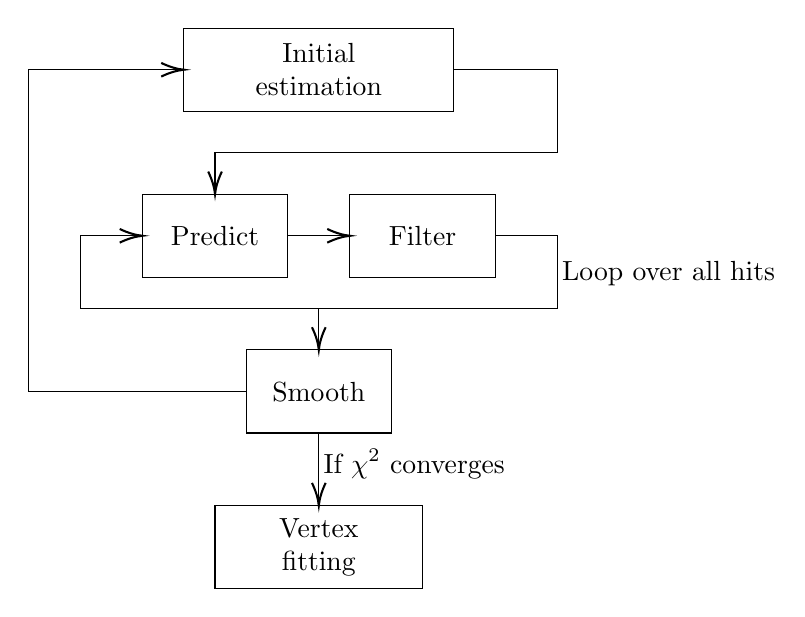
\begin{tikzpicture}[x=0.75pt,y=0.75pt,yscale=-1,xscale=1]
	%uncomment if require: \path (0,359); %set diagram left start at 0, and has height of 359

	%Shape: Rectangle [id:dp9978340606054834] 
	\draw   (205,20) -- (335,20) -- (335,60) -- (205,60) -- cycle ;
	%Shape: Rectangle [id:dp36333722789056344] 
	\draw   (185,100) -- (255,100) -- (255,140) -- (185,140) -- cycle ;
	%Shape: Rectangle [id:dp8065489263231345] 
	\draw   (285,100) -- (355,100) -- (355,140) -- (285,140) -- cycle ;
	%Shape: Rectangle [id:dp3416154088376071] 
	\draw   (235,175) -- (305,175) -- (305,215) -- (235,215) -- cycle ;
	%Shape: Rectangle [id:dp4411494772649741] 
	\draw   (220,250) -- (320,250) -- (320,290) -- (220,290) -- cycle ;
	%Straight Lines [id:da7344533518933397] 
	\draw    (335,40) -- (385,40) -- (385,80) -- (220,80) -- (220,98) ;
	\draw [shift={(220,100)}, rotate = 270] [color={rgb, 255:red, 0; green, 0; blue, 0 }  ][line width=0.75]    (10.93,-3.29) .. controls (6.95,-1.4) and (3.31,-0.3) .. (0,0) .. controls (3.31,0.3) and (6.95,1.4) .. (10.93,3.29)   ;
	%Straight Lines [id:da06782376989613081] 
	\draw    (255,120) -- (283,120) ;
	\draw [shift={(285,120)}, rotate = 180] [color={rgb, 255:red, 0; green, 0; blue, 0 }  ][line width=0.75]    (10.93,-3.29) .. controls (6.95,-1.4) and (3.31,-0.3) .. (0,0) .. controls (3.31,0.3) and (6.95,1.4) .. (10.93,3.29)   ;
	%Straight Lines [id:da03444837242423393] 
	\draw    (355,120) -- (385,120) -- (385,155) -- (155,155) -- (155,120) -- (183,120) ;
	\draw [shift={(185,120)}, rotate = 180] [color={rgb, 255:red, 0; green, 0; blue, 0 }  ][line width=0.75]    (10.93,-3.29) .. controls (6.95,-1.4) and (3.31,-0.3) .. (0,0) .. controls (3.31,0.3) and (6.95,1.4) .. (10.93,3.29)   ;
	%Straight Lines [id:da9288077865829715] 
	\draw    (270,155) -- (270,173) ;
	\draw [shift={(270,175)}, rotate = 270] [color={rgb, 255:red, 0; green, 0; blue, 0 }  ][line width=0.75]    (10.93,-3.29) .. controls (6.95,-1.4) and (3.31,-0.3) .. (0,0) .. controls (3.31,0.3) and (6.95,1.4) .. (10.93,3.29)   ;
	%Straight Lines [id:da9916095919187531] 
	\draw    (235,195) -- (130,195) -- (130,40) -- (203,40) ;
	\draw [shift={(205,40)}, rotate = 180] [color={rgb, 255:red, 0; green, 0; blue, 0 }  ][line width=0.75]    (10.93,-3.29) .. controls (6.95,-1.4) and (3.31,-0.3) .. (0,0) .. controls (3.31,0.3) and (6.95,1.4) .. (10.93,3.29)   ;
	%Straight Lines [id:da7888302009088826] 
	\draw    (270,215) -- (270,248) ;
	\draw [shift={(270,250)}, rotate = 270] [color={rgb, 255:red, 0; green, 0; blue, 0 }  ][line width=0.75]    (10.93,-3.29) .. controls (6.95,-1.4) and (3.31,-0.3) .. (0,0) .. controls (3.31,0.3) and (6.95,1.4) .. (10.93,3.29)   ;

	% Text Node
	\draw (270,40) node   [align=left] {\begin{minipage}[lt]{72.76pt}\setlength\topsep{0pt}
			\begin{center}
				Initial estimation
			\end{center}

		\end{minipage}};
	% Text Node
	\draw (220,120) node   [align=left] {\begin{minipage}[lt]{34pt}\setlength\topsep{0pt}
			\begin{center}
				Predict
			\end{center}

		\end{minipage}};
	% Text Node
	\draw (320,120) node   [align=left] {\begin{minipage}[lt]{24.48pt}\setlength\topsep{0pt}
			\begin{center}
				Filter
			\end{center}

		\end{minipage}};
	% Text Node
	\draw (270,195) node   [align=left] {\begin{minipage}[lt]{37.4pt}\setlength\topsep{0pt}
			\begin{center}
				Smooth
			\end{center}

		\end{minipage}};
	% Text Node
	\draw (270,270) node   [align=left] {\begin{minipage}[lt]{55.76pt}\setlength\topsep{0pt}
			\begin{center}
				Vertex fitting
			\end{center}

		\end{minipage}};
	% Text Node
	\draw (386,131) node [anchor=north west][inner sep=0.75pt]   [align=left] {Loop over all hits};
	% Text Node
	\draw (271,230) node [anchor=west] [inner sep=0.75pt]   [align=left] {If $\displaystyle \chi ^{2}$ converges};


\end{tikzpicture}


	\caption{Flow chart of Kalman filter algorithm for track fitting.}
	\label{fig:kalman_flowchart}
\end{figure}

\begin{figure}
	\centering
	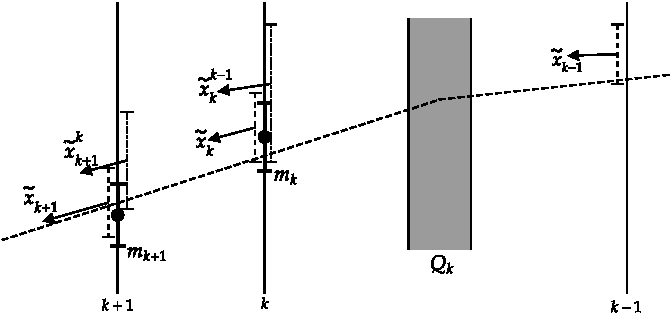
\includegraphics[width=0.8\linewidth]{kalman_node}
	\caption{Schematic representation of Kalman filter workflow. The predicted and measured hit location
		are denoted as $\tilde{x}^i_j$ and $m_j$ respectively. The estimated location on the $j$-th plane
		are calculated on the state variables from the $i$-th detector plane. The combined estimate of the
		state variable $\tilde{x}_j$ are then calculated by comparing the $\tilde{x}^i_j$ and $m_j$.}
	\label{fig:kalman_node}
\end{figure}

\subsection{Vertex Finding}
Once all the tracks are found in each event, the reconstruction of the dimuon vertex can begin using kVertex.
For MATRIX-1 events, all possible combinations of $\mu^+$ and $\mu^-$ tracks are tested if they can form
a dimuon. The vertex is determined using the same Kalment filter with the tracks acting as measurements.

\pdfmargincomment{kalment filter, refitting if it the pair originate from target to account for multiple scattering }
To account for multiple scattering of the muons while traversing FMag, dimuon pairs that are
determined to be likely originating from the target, are refitted by requiring the dimuon vertex to
fall within the target. Due to the length of the target and the acceptance of the spectrometer,
the most probable z-vertex is found to depend on the mass of the dimuon, and is calculated from the
following empirical formula~\cite{kun-1283}
\begin{equation}
	z\left(m\right) = -199.332 + 27.9488 m - 3.66186 m^2 + 0.175479 m^3.
\end{equation}
The refitting procedure is repeated until the new z-vertex reaches convergence.


\subsection{Dimuon Kinematic Variables}
\label{subsec:def_kinematic}
The dimuon kinematic variable is calculated after vertex finding. The primary outputs of kTracker
are the four-momenta of the two muons as well as the dimuon vertex. The other variables are inferred
from these information. While most variables have consistent definitions across literature, the momentum
fractions $x_1$, $x_2$ and the Feynman x ($x_F$) require some attentions as there can be multiple definitions.

Feynman x, or $x_F$, is defined as $P_z/P_z^{max}$, the ratio of longitudinal dimuon momentum
over the maximum allowed value in the hadron-hadron center of mass frame. In high energy
experiment, $P_z^{max}$ is often given as $\sqrt{s}/2$, since half of the available energy is
carried away by the recoiled system.
However, as SeaQuest is at a lower energy, the mass of the virtual photon becomes comparable to its momentum.
A heavier virtual photon would imply less available energy for the longitudinal momentum,
therefore we defined $x_F$ as
\begin{equation}
	x_F = \frac{2P_z}{\sqrt{s}-M^2/\sqrt{s}},
\end{equation}
where $M$ is the dimuon mass.

For the momentum fractions $x_1$, $x_2$, the following definition, taken from Ref.~\cite{Coester-1286} is chosen
\begin{equation}
	\begin{split}
		x_1 &= \frac{P_{\textrm{target}}\cdot P_{\gamma^*}}{P_{\textrm{target}}\cdot (P_{\textrm{beam}}+P_{\textrm{target}})},\\
		x_2 &= \frac{P_{\textrm{beam}}\cdot P_{\gamma^*}}{P_{\textrm{beam}}\cdot (P_{\textrm{beam}}+P_{\textrm{target}})},
	\end{split}
\end{equation}
where $P_{\textrm{beam}}$, $P_{\textrm{target}}$ and $P_{\gamma^*}$ are the four momentum of the
beam hadron, target hadron and the virtual photon respectively.

Because of our choice of $x_1$, $x_2$ definitions, the mass of the dimuon is now related to
the momentum fractions as
\begin{equation}
	M^2= sx_1x_2-P_T^2.
\end{equation}
And $x_F$ is no longer the difference between $x_1$ and $x_2$.

Other definitions of the momentum fractions are listed in \cref{M-a_ch:kinematic}. These different definitions
are consistent in the limit of zero dimuon transverse momentum.
Neglecting the small intrinsic momentum of the partons,
the transverse momentum of the virtual photon mostly originates from higher order QCD effect, such as gluon
emission by the quarks. Therefore, a virtual photon with large transverse momentum would originate
from partons with higher energy than the longitudinal dimuon momentum alone would suggest. The different
definitions differ on how they attribute the transverse momentum to the partons.

\section{Background Simulation}
\label{sec:mixing}
To obtain the profile of the accidental background, a track-mixing method is adopted.
We believe the accidental background is coming from the decay of multiple pions created from multiple interactions
within the same RF buckets. By combining two uncorrelated muon tracks, we can simulate the profile
of the accidental background.

The chosen method in our group is by mixing tracks from MATRIX-4 events. The MATRIX-4 triggers when
only one muon track is observed in the spectrometer.
The accidental background template is then created by combining a $\mu^+$ track with
another $\mu^-$ track from a different event. This method is first studied by
J.~Dove~\cite{dove2020}.

The MATRIX-4 events are first processed by the same track finding procedure as with
the MATRIX-1 dimuon data.
To reproduce the MATRIX-1 trigger requirements, the MATRIX-4 tracks are then separated in bins
based on the charge and top/bottom halves of the spectrometer. Since the MATRIX-1
requires the two opposite tracks to be on different halves on the spectrometer,
a positive tracks in the top half would only be mixed with a negative tracks in the
bottom half of the spectrometer, and vice versa. The MATRIX-4 data is also separated
based on the target position. During the mixing procedure, only the tracks from same
target would be analyzed together.
The data can also optionally be binned in the occupancy to study the intensity dependence
of the accidental background.

In order to preserve any change in performance in the spectrometer over time, all the
MATRIX-4 tracks in each bin are then sorted in time. Tracks are then mixed in chronological order.
While MATRIX-4 triggers on a single track, it is also
possible for the reconstruction software to find multiple tracks in a given MATRIX-4 event.
In order to prevent tracks from the same event to be mixed, a sliding number $d$ can also be introduced.
With this option enabled, the $i$-th positive track would be mixed with the $\left(i+d\right)$-th negative track.
Typically, a sliding number of one is chosen.
A minor benefit is that this method also ensures the result to be reproducible as compared to random
mixing.

Once the two tracks are selected, the mixed events are ready for vertex finding. As with the
real data, the dimuon kinematics variables are calculated. The same dimuon selection will
also be applied and can be compared with the real data. Since the probability of observing a
single track event is much higher than a two track event, the MATRIX-4 trigger is typically
heavily prescaled to preserve DAQ bandwidth. Typically, a prescale factor of \num{30000} is used during
normal data taking run, meaning only \num{1} in \num{30000} single track event is recorded.
Therefore, the amount of available MATRIX-4 data for each target can be limited. The mixed events
from different target can also be combined to increase statistics. For this study, the \ce{LH_2}
and \ce{LD_2} mixed events are combined during the mass fitting.

Alternative accidental background generating methods have also been proposed by different groups.
One such method is proposed by K. Liu. In this method, MATRIX-1 events are used. In order to track the
change of the spectrometer performance over time, two tracks from the same 1 hour run are selected
randomly. The two tracks are still required to fulfill the opposite charge and top/bottom requirements.
The two tracks are also required to have similar occupancy, usually within \SI{10}{\percent}.
Because of the use of MATRIX-1 data, the mixed sample has larger statistics. Therefore, when
using MATRIX-1 mixed sample, target specific mixed sample is typically used. One disadvantage to using MATRIX-1
was potential contamination from physics sources. For example, near the $J/\psi$ peak, the MATRIX-1
data is heavily dominated by the charmonium decay, therefore it is possible that both tracks in the same
mixed event are from the $J/\psi$ decay. While it is possible to have multiple $J/\psi$ decays or
multiple Drell-Yan interactions in the same RF bucket,
the probability is relatively small. It is more likely to have multiple pions produced in the same RF
buckets by multiple interactions, which then decay into high energy muons, forming a high-mass
dimuon background.
On the contrary, the MATRIX-4 trigger fires when there is only one track, and therefore less
susceptible to the contamination from physics sources.

Both mixing samples are used for the mass fit studies and the difference is quoted as a source systematic
uncertainty.

\section{Dimuon Selection}
The event selection that is used in this study is based on the study by C.~Brown~\cite{chuck-2111}
with some modification to increase acceptance at low mass. These cuts
are categorized into different groups and are tabulated in \cref{table:trackCut,table:dimuonCut,table:physCut,table:occCut}.

\renewcommand{\thefootnote}{\fnsymbol{footnote}}
\begin{table}[ht!]
	\centering
	\caption{Track level cuts.}
	\label{table:trackCut}
	\begin{tabular}{|m{4.5cm}|m{7cm}|m{3cm}|}
		\hline
		Variable                                                                                                                                                                                     & Description                                                                          & Cut                          \\ \hline
		$\chi^2_{\mathrm{target}}$                                                                                                                                                                   & $\chi^2$ when track is   forced to pass through center of target ($z=\SI{-129}{\cm}$) & $< 15$                       \\ \hline
		$pz_1$                                                                                                                                                                                       & z momentum at station 1                                                              & (\SI{9}{\GeV},\SI{75}{\GeV}) \\ \hline
		nHits                                                                                                                                                                                        & total number of hits on wire chambers by each   muon track                           & $> 13$                       \\ \hline
		$x_T^2 +(y_T - \mathrm{beamOffset})^2$                                                                                                                                                       & radial distance of track from   beam line at the center of target                    & $< \SI{320}{\cm\squared}$    \\ \hline
		$x_D^2 +(y_D - \mathrm{beamOffset})^2$                                                                                                                                                       &
		radial distance of track from   beam line at the center of beam dump ($z=\SI{42}{\cm}$)                                                                                                      &
		(\SI{8}{\cm\squared},\SI{1100}{\cm\squared})   \footnotemark[1]                                                                                                                                                                                                                                                    \\ \hline
		\begin{tabular}[c]{@{}c@{}}$\chi^2_{\mathrm{target}}<1.5\chi^2_{\mathrm{upstream}}$\\      $\chi^2_{\mathrm{target}}<1.5\chi^2_{\mathrm{dump}}$\end{tabular} &
		$\chi^2$ when track is   forced to pass through $z=\SI{-490}{\cm}$(upstream), $z=\SI{-129}{\cm}$(traget) and   $z=\SI{42}{\cm}$(dump)                                                         &
		\\ \hline
		$z_0$                                                                                                                                                                                        & z position of track's closest approach to beam   line                                & (\SI{320}{\cm},\SI{-5}{\cm}) \\ \hline
		$\chi^2/(\mathrm{nHits}-5)$                                                                                                                                                                  & $\chi^2/\mathrm{ndf}$                                                                & $<12$                        \\ \hline
		$y_1/y_3$                                                                                                                                                                                    & y position of track at St.~1   and St.~3                                            & $<1$                         \\ \hline
		$y_1\times y_3$                                                                                                                                                                              &                                                                                      & $>0$                         \\ \hline
		$| |px_1 - px_3| -0.416|$                                                                                                                                                                    & difference in x momentum at St.~1 and St.~3 accounting for the Kmag kick             & $<\SI{0.008}{\GeV}$          \\ \hline
		$|py_1 - py_3|$                                                                                                                                                                              & difference in y momentum at St.~1 and St.~3                                          & $<\SI{0.008}{\GeV}$          \\ \hline
		$|pz_1 - pz_3|$                                                                                                                                                                              & difference in z momentum at St.~1 and St.~3                                          & $<\SI{0.08}{\GeV}$           \\ \hline
		$|py_1 |$                                                                                                                                                                                    & absolute value of the y momentum   at St.~1                                          & $>\SI{0.02}{\GeV}$           \\ \hline
	\end{tabular}
\end{table}

\begin{table}[ht!]
	\centering
	\caption{dimuon level cuts.}
	\label{table:dimuonCut}
	\begin{tabular}{|m{4.5cm}|m{7cm}|m{3cm}|}
		\hline
		Variable                                                                                                                          & Description                                                                              & Cut                            \\ \hline
		$|dx|$                                                                                                                            & x position of dimuon vertex                                                              & $<\SI{0.25}{\cm}$              \\ \hline
		$|dy-\mathrm{beamOffset}|$                                                                                                        & y position of dimuon vertex                                                              & $<\SI{0.22}{\cm}$              \\ \hline
		$dz$                                                                                                                              & z position of dimuon vertex                                                              & (\SI{-280}{\cm},\SI{-5}{\cm})  \\ \hline
		$dx^2+(dy-\mathrm{beamOffset})^2$                                                                                                 & radial distance of the dimuon vertex from beam line                                      & $<\SI{0.06}{\cm\squared}$      \\ \hline
		$|dpx|$                                                                                                                           & absolute value of dimuon x   momentum                                                    & $<\SI{1.8}{\GeV}$              \\ \hline
		$|dpy|$                                                                                                                           & absolute value of dimuon y   momentum                                                    & $<\SI{2}{\GeV}$                \\ \hline
		$dpx^2+dpy^2$                                                                                                                     & transverse momentum squared of   dimuon                                                  & $<\SI{5}{\GeV}$                \\ \hline
		dpz                                                                                                                               & dimuon z momentum                                                                        & (\SI{38}{\GeV},\SI{116}{\GeV}) \\ \hline
		$|\mathrm{tackSeparation}|$                                                                                                       & distance in z between points   of  closest approach between $\mu^+$   and $\mu^-$ track  & $<\SI{270}{\cm}$               \\ \hline
		$\chi^2_{\mathrm{dimuon}}$                                                                                                        & $\chi^2$ when both $\mu^+$ and   $\mu^-$ tracks are forced to pass through dimuon vertex & $<18$                          \\ \hline
		$\begin{aligned} |\chi^2_{\mathrm{target}}(\mu^+) &+ \chi^2_{\mathrm{target}}(\mu^-)\\& -\chi^2_{\mathrm{dimuon}}| \end{aligned}$ &                                                                                          & $<2$                           \\ \hline
		$y_3(\mu^+) \times y_3(\mu^-)$                                                                                                    & y position at St.~3 for both tracks                                                      & $<0$                           \\ \hline
		$\mathrm{nHists}(\mu^+)+\mathrm{nHists}(\mu^-)$                                                                                   & sum of the total number if hits on wire chamber by $\mu^+$ and $\mu^-$ track             & $>29$                          \\ \hline
		$\mathrm{nHists}_1(\mu^+)+\mathrm{nHists}_1(\mu^-)$                                                                               & sum of the total number if hits on St.~1 wire chamber by $\mu^+$ and $\mu^-$ track       & $>8$                           \\ \hline
		$|x_1(\mu^+) + x_1(\mu^-)|$                                                                                                       & sum off x position of of tracks   at St.~1                                               & $>\SI{42}{\cm}$                \\ \hline
	\end{tabular}
\end{table}

\begin{table}[h!]
	\centering
	\caption{ physics cuts}
	\label{table:physCut}
	\begin{tabular}{|m{4.5cm}|m{7cm}|m{3cm}|}
		\hline
		Variable              & Description                          & Cut                                                            \\ \hline
		mass                  & dimuon mass                          & (\SI{2}{\GeV},\SI{8.8}{\GeV}) \footref{fn:chuck}\tablefootnote{The 0.99 scaling factor is applied to MC} \\ \hline
		$x_F$                 & Feynman $x$                          & (-0.1,0.95)                                                    \\ \hline
		$x_{\mathrm{target}}$ & Bjorken $x$ of target                & (0.005,0.55) \footref{fn:chuck}                                \\ \hline
		$|\cos(\theta)|$      & polar angle in Collins-Soper   frame & $<0.5$                                                         \\ \hline
	\end{tabular}
\end{table}
\begin{table}[h!]
	\centering
	\caption{occupancy cuts}
	\label{table:occCut}
	\begin{tabular}{|m{4.5cm}|m{7cm}|m{3cm}|}
		\hline
		Variable                          & Description                                & Cut      \\ \hline
		D1                                & total hits on St.~1 Chamber                & $<400$   \\ \hline
		D2                                & total hits on St.~2 Chamber                & $<400$   \\ \hline
		D3                                & total hits on St.~3 Chamber                & $<400$   \\ \hline
		$D1+D2+D3$                        & total numbers of hits in all wire Chambers & $<1000$  \\ \hline
		Trigger intensity\tablefootnote{Not applied to MC or Mix background} & numbers of proton in the triggering bucket & $<80000$ \\ \hline
	\end{tabular}
\end{table}


%\footnotetext[1]{modified from Ref.~\cite{chuck-2111}}
%\footnotetext[2]{The 0.99 scaling factor is applied to MC}
%\footnotetext[3]{Not applied to MC or Mix background}
\FloatBarrier
\section{Beam Luminosity Normalization}\pdfmargincomment{might move this section to spectrometer}
\label{sec:beam_norm}
In SeaQuest, there are three beam luminosity related quantities.
During data taking, the proton on target is monitored by two sets of instruments, a secondary
emission monitor located upstream of the SeaQuest experimental hall, and a Cherenkov counter
(as described in \cref{M-subsec:BIM}). The secondary emission monitor provides the integrated
beam intensity for the entire beam spill (labeled as ``G2SEM"). This is sometimes referred as
``raw proton'' as this quantity does not include any deadtime or inhibit effect.

The Cherenkov counter provides the beam intensity for each RF bucket in relative units.
During normal data taking, the Beam DAQ records three quantities: integrated beam intensity for entire spill
(labeled as ``QIEsum''), integrated beam while inhibit is asserted at trigger logic
(labeled as ``inhibit\_block\_sum'') and integrated intensity during dead time (labeled as
``trigger\_sum\_no\_inhibit''). All these quantities are in relative units.

In previous studies, the number of protons on targets during DAQ live time can be calculated as follows:
\begin{equation}
	\mathrm{live\ proton} = \frac{\mathrm{QIEsum}-\mathrm{inhibit\_block\_sum}-\mathrm{trigger\_sum\_no\_inhibit}}{\mathrm{QIEsum}}\cdot \mathrm{G2SEM}
	\label{eq:livePoT-old}
\end{equation}
The conversion factor from QIE units to number of proton ($\frac{\mathrm{G2SEM}}{\mathrm{QIEsum}}$)
is also a function of time. This is due to radiation damage to the mirror. The mirror needs to be replaced
regularly. This factor over time is shown in \cref{fig:potperQIE}.
\begin{figure}
	\centering
	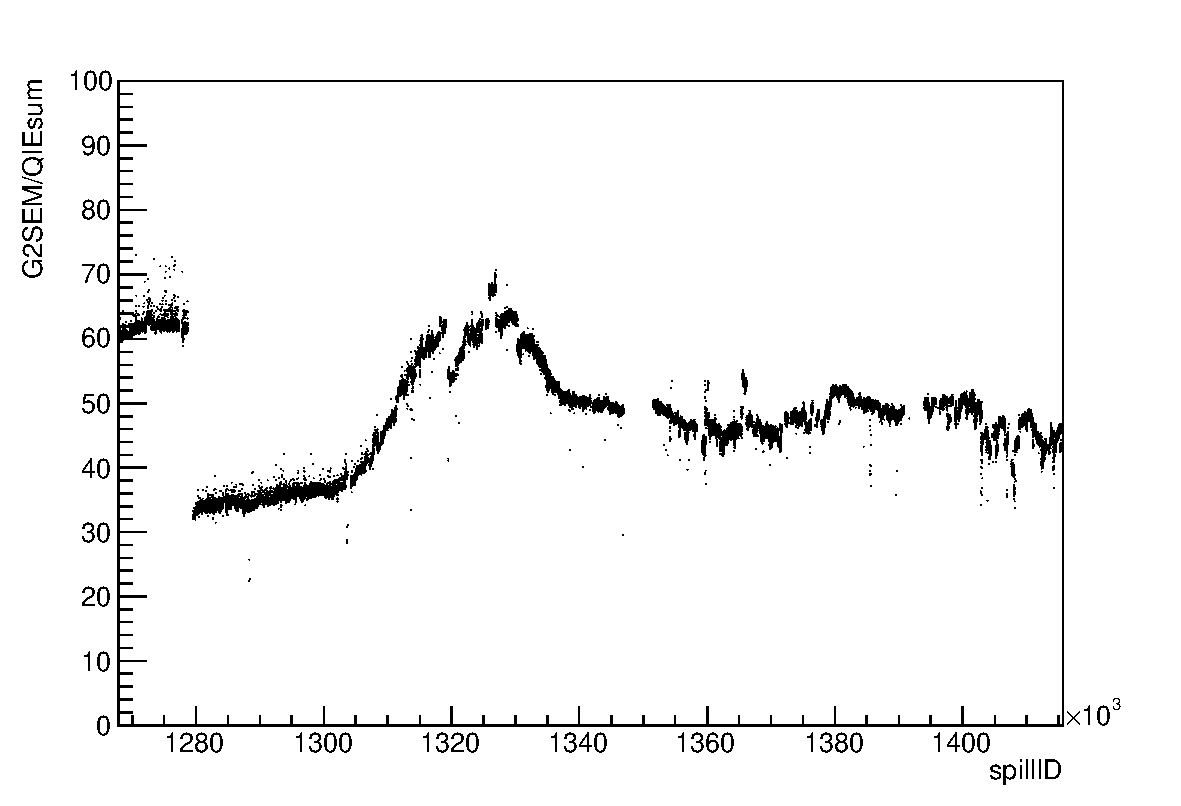
\includegraphics[width=0.5\linewidth]{run6_LH2_potPerQIE}
	\caption{The conversion factor from QIE units to number of proton over time.}
	\label{fig:potperQIE}
\end{figure}

However, there is a pedestal in the QIE measurements. This is partly originate from the dark rate of the 
detector. And this pedestal needs to be subtracted from the sums. 
The value of the pedestal is obtained by studying empty buckets. 
This value can change over time and is summarized in \cref{tabel:pedestal}.
A typical spill contains $588\cdot 369000$ buckets, hence the $\mathrm{QIEsum}$ should be replaced with
\begin{equation}
	\mathrm{QIEsum}-\mathrm{pedestal}\cdot 588\cdot 369000.
\end{equation}
However, the numbers of bucket during DAQ deadtime or while the inhibit is asserted are less clear,
as they are not always recorded reliably~\cite{chleung-10662}.
Instead, the number of buckets during the DAQ deadtime of the whole dataset 
is estimated using the measured deadtime from run periods where we believe the measurements are reliable.
The measured deadtime per event for Run 5 is shown in \cref{fig:deadtime}.
The extracted mean deadtime is used for the analysis of Run 2-3 and Run 5 data. 
For Run 6, due to the DAQ upgrade, the deadtime is reduced to a fixed \SI{29.5}{\us}.
The number of buckets during deadtime is estimated as
\begin{equation}
	N_{\mathrm{busy\ RF}}=N_{\mathrm{trigger}}\times\frac{\expval{\mathrm{deadtime}}}{18.9\unit{\ns}},
\end{equation}
where $N_{\mathrm{trigger}}$ is the number of trigger during a spill, and \SI{18.9}{\ns} is the width of a bucket. 
Therefore, the $\mathrm{busy\_sum\_no\_inhibit}$ is \cref{eq:livePoT-old} is replaced by
\begin{equation}
	\mathrm{busy\_sum\_no\_inhibit} - N_{\mathrm{busy\ RF}}\cdot \mathrm{pedestal}.
\end{equation}
\begin{figure}[h!]
	\centering
	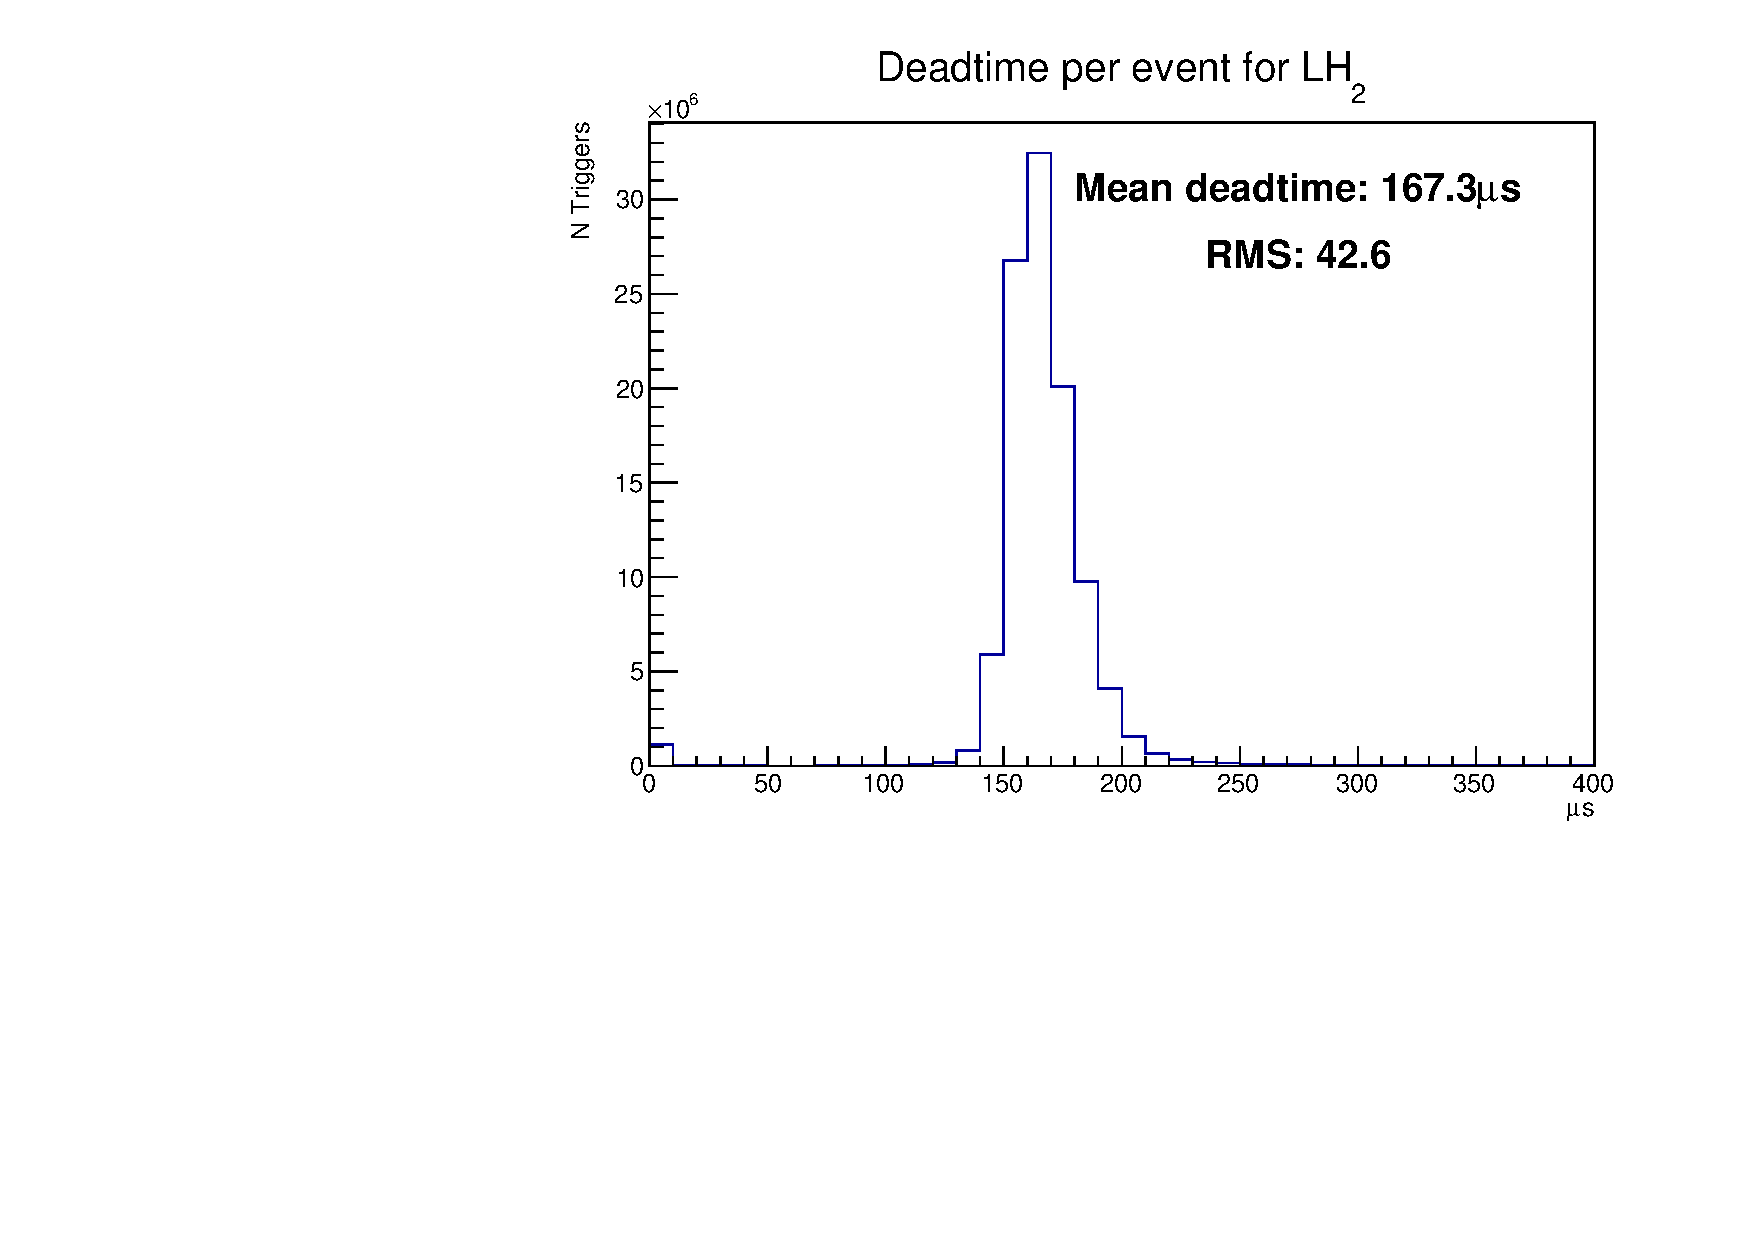
\includegraphics[width=0.6\linewidth]{run5ea_deadtime}
	\caption{The measured deadtime per event for \ce{LH_2} target from Run 5.}
	\label{fig:deadtime}
\end{figure}

During regular data-taking, the minimum width of the inhibit signal is control by a programmable
register, and is typically set to 16, meaning when bucket $i$ is above the threshold, bucket $i-8$
to $i+8$ (inclusive) with be inhibited. The length of the inhibit can be longer if a series
of high intensity buckets arrive in succession. In this situation, the inhibit will extend till 8
buckets after the last high intensity bucket. However, the length of each inhibit is not always available.
Hence the number of inhibited buckets is estimated using the minimum inhibit width.
\begin{equation}
	N_{\mathrm{inhibited\ RF}}=N_{\mathrm{inhibit}}\cdot 17,
\end{equation}
where $N_{\mathrm{inhibit}}$ is the number of inhibit asserted.
And the $\mathrm{inhibit\_block\_sum}$ is replaced by
\begin{equation}
	\mathrm{inhibit\_block\_sum}-N_{\mathrm{inhibited\ RF}}\cdot\mathrm{pedestal}.
\end{equation}

Therefore the pedestal-corrected live proton is given by
\begin{multline}
	\frac{\mathrm{live\ proton}}{\mathrm{G2SEM}}= 1-\frac{1}{\mathrm{QIEsum}-\mathrm{pedestal}\cdot 588\cdot 369000}\times\big[\mathrm{inhibit\_block\_sum}\\
	+\mathrm{trigger\_sum\_no\_inhibit}-\mathrm{pedestal}\cdot\left(N_{\mathrm{inhibited\ RF}}+N_{\mathrm{busy\ RF}}\right)\big].
	\label{eq:livePoT-new}
\end{multline}
This pedestal correction is found to have $\sim 5-10\%$ effect on the absolute normalization,
but negligible effects on the relative normalization~\cite{chleung-10679}.


The Main DAQ also reads out the beam intensity from Cherenkov counter for the triggering bucket
and the $\pm16$ RF buckets before and after the trigger (label as ``RF-16" to ``RF+16", with
``RF00'' being the triggering bucket).

The number of proton in the triggering bucket can be calculated as follows:
\begin{equation}
	\mathrm{trigger\ intensity} = \frac{\mathrm{RF00}-\mathrm{pedestal}}{\mathrm{QIEsum}-\mathrm{pedestal}\cdot 588\cdot 369000}\cdot \mathrm{G2SEM}
\end{equation}
\begin{table}[h!]
	\centering
	\caption{Summary of the QIE pedestal over time\cite{kenichi-9289}.}
	\label{tabel:pedestal}
	\begin{tabular}{|c|c|c|}
		\hline
		Run     & spill range                     & pedestal value \\ \hline
		2-3     &                                 & $34\pm5$       \\ \hline
		5       & $[\num{910000},\num{1010000})$  & $33\pm 6$      \\ \cline{2-3}
		        & $[\num{1010000},\num{1100000})$ & $28\pm 5$      \\ \hline
		6       & $[\num{1200000},\num{1320000})$ & $40\pm 12$     \\ \cline{2-3}
		        & $[\num{1320000},\num{1420000})$ & $30\pm 7$      \\ \hline
	\end{tabular}
\end{table}

\section{Mass Spectrum Fitting}
With the goal of obtaining the absolute yield for different processes, the mass spectrum fitting
procedure is developed. This also forms the bases of our recent publication~\cite{dove2023}.

The event distribution can be expressed as a linear combination of different components,
namely Drell-Yan, charmonium decays, accidental background and background from instruments.
These different contributions would have distinct mass spectra, for example, the $J/\psi$
and $\psi^\prime$ decays would have sharp distributions centered around their masses.
Therefore, the data can be fitted to various templates to obtain
the relative contribution from each sources.

\paragraph{Physics sources}
The templates for $J/\psi$, $\psi'$ and Drell-Yan are obtained by analyzing the messy Monte Carlo
simulation (as described in \cref{subsec:messyMC}). The same analysis cuts are applied to both data
and messy Monte Carlo.

\paragraph{Empty flask subtraction}
The empty flask data is taken by placing just the empty flask (without air inside) in the path of
the beam. It is used for understanding the background originating from interactions of the beam
with the flask wall, beam dump or various upstream instrumentation. The normalization of the
empty flask contribution is obtained from the ratio of live protons for the liquid target and
empty flask. The empty flask normalization is then kept fixed during the fitting procedure, while
other components are allowed to float. The relative live proton ratio is used for the normalization here, as the
mass distribution is obtained by integrating over intensity, and rate dependence effect will need
to be corrected later.

\paragraph{Accidental/Mixed background correction}
As described in \cref{sec:mixing}, the mixed sample from the MATRIX-4 is typically used.
Due to the limited sample size in the raw MATRIX-4 data, 
the statistics of the mixed sample is typically limited. For both \ce{LH_2} and \ce{LD_2} studies, 
the mixed sample from both \ce{LH_2} and \ce{LD_2} are combined.
Then the sample template is used for both \ce{LH_2} and \ce{LD_2} analysis.
Other mixed samples can also be used. This is done to estimate the systematic uncertainty.

\subsection{TFractionFitter}
To account for the statistical uncertainties in both the data and Monte Carlo
simulation, the TFractionFitter algorithm~\cite{barlow1993} is used in this analysis.
This is achieved by performing a standard likelihood fit using Poisson statistics,
while the templates, generated from MC, are also varied within statistics, leading
to additional contributions to the overall likelihood.

Let there be $m$ sources, the number of MC events in bin $i$ from source $j$
is given by $a_{ji}$. For each source, there is some (unknown) expected distribution
$A_{ji}$. The expected number of events in each bin is given by
\begin{equation}
	f_i = \sum^m_{j=1} p_j A_{ji}.
	\label{eq:TF_f}
\end{equation}
From each $A_{ji}$, the number of Monte Carlo events $a_{ji}$ is obtained.
The total likelihood is the combined probability of the number of observed events $\left\{d_i\right\}$
and the number of MC events $\left\{a_{ji}\right\}$
\begin{equation}
	\ln \mathcal{L} = \sum^n_{i=1} \left(d_i \ln f_i -f_i\right) + \sum^n_{i=1} \sum^m_{j=1} \left(a_{ji} \ln A_{ji} - A_{ji}\right).
	\label{eq:TF_likelihood}
\end{equation}
The estimates for the strength $p_j$ and the expected distribution $A_{ji}$ are
found by maximizing this likelihood. One consequence of this approach is the addition of
$n \cross m$ fit parameters $A_{ji}$. However, the  minimization of these additional
parameters is done analytically rather than treating them as formal fit parameters.

To maximize the likelihood, \cref{eq:TF_likelihood} is differentiated with respect to $p_j$ 
and $A_{ji}$ and the derivatives are set to zero.
This yields two sets of equations, those for the differentials with respect to $p_j$,
\begin{equation}
	\sum^n_{i=1} \left(\frac{d_i A_{ji}}{f_i} -A_{ji}\right)=0\quad \forall j,
	\label{eq:TF_d1}
\end{equation}
and those for the differentials with respect to $A_{ji}$
\begin{equation}
	\frac{d_i p_j}{f_i} - p_j + \frac{a_{ji}}{A_{ji}}-1=0\quad \forall 	i,j.
	\label{eq:TF_d2}
\end{equation}
\Cref{eq:TF_d2} and be simplified by rewritten as 
\begin{equation}
	1-\frac{d_i}{f_i} = \frac{1}{p_j}\left(\frac{a_{ji}}{A_{ji}}-1\right)\quad \forall i,j.
	\label{eq:TF_d3}
\end{equation}
Since the left hand side only depends on $i$, one can define $t_i$ as
\begin{equation}
	t_i= 1-\frac{d_i}{f_i}.
	\label{eq:TF_d4}
\end{equation}
And the right hand side can expressed as 
\begin{equation}
	A_{ji}=\frac{a_{ji}}{1+p_j t_i}.
\end{equation}
This reduces the $m\cross \left(n+1\right)$ unknowns in \cref{eq:TF_likelihood} ($p_j$ and $A_{ji}$)
into $m+n$ unknowns ($p_j$ and $t_i$).
And \cref{eq:TF_f} and be expressed as
\begin{equation}
	\frac{d_i}{1-t_i}=f_i=\sum_j^m p_jA_{ji}=\sum_j^m \frac{p_j a_{ji}}{1+p_jt_i}.
	\label{eq:TF_d5}
\end{equation}
To solve for $p_j$ and $t_i$, one can employ an interactive procedure. First, solve for $p_j$ by maximizing
\cref{eq:TF_d1} using numerical methods with fixed $t_i$. Next, refine $t_i$ by using \cref{eq:TF_d5} while keeping
$p_j$ fixed. Repeat the process until convergence is reached.

Some nice features arises automatically from the algebra. Substituting \cref{eq:TF_d3} into \cref{eq:TF_d1},
\begin{equation}
	\sum_{i=1}^{n} A_{ji}=\sum_{i=1}^{n} a_{ji}\quad\forall j .
\end{equation}
These means the estimate of $A_{ji}$ for some source $j$ will change the shape of the distribution
from that of the MC data $a_{ji}$, but will preserve the overall total number. 

Using \cref{eq:TF_d2} and summing over $i$ and $j$, 
\begin{equation}
	\sum_{i=1}^n d_i = \sum_{i=1}^{n}\sum_{j=1}^m p_j a_{ji},
\end{equation}
which returns the normalization, without the need for imposing additional constraints.

In the case of weighted MC, \cref{eq:TF_f} would need to be modified into
\begin{equation}
	f_i = \sum^m_{j=1} p_j w_{ji}A_{ji},
\end{equation}
where $w_{ji}$ is the average weight of the MC events in bin $i$ from the source $j$.
And $A_{ji}$ is given by
\begin{equation}
	A_{ji}=\frac{a_{ji}}{1+p_j w_{ji}t_i}.
\end{equation}

\subsection{Yield Extraction}
The normalization for different components (except for empty flask, which is fixed by relative live proton ratio)
can obtained by fitting to the mass distribution. Once the normalization is obtained, the yield can be
obtained. To minimize the impact of the Monte Carlo input to the extracted Drell-Yan yield, the Drell-Yan Monte
Carlo is only used during the fitting procedure. And the Drell-Yan yield is defined as follows
\begin{equation}
	Y_{DY}= N_{\textrm{data}}-p_{J/\psi} N_{J/\psi}-p_{\psi'} N_{\psi'}-p_{mix bkg.} N_{mix bkg.} - p_{\textrm{flask}} N_{\textrm{flask}},
\end{equation}
where the $p_a$ is the scale factor for each component $a$. $p_{\textrm{flask}}$ is obtained from the
ratio of live proton between the target of interest and the empty flask,
whereas the scale factor for the other components are obtained from the fitting procedure.
In the case of Monte Carlo, $N$ is the weighted integral of the
simulated distribution, whereas $N_{mix bkg.}$ and $N_{\textrm{flask}}$ are the number of events in the mixed
sample and empty flask data.

For the charmonium studies, we can utilized the fact that they are resonances and show up as distinct peaks
in the mass spectrum. A separate mass fit can be performed for each kinematic bin. Since each bin is analyzed
separately, the input Monte Carlo would have little effect on the extract yield. Therefore the yield is simply
\begin{equation}
	Y_{J/\psi}= p_{J/\psi} N_{J/\psi}.
\end{equation}
One downside of such approach is that the kinematic bin would need to be sufficiently wide to ensure enough
data across a wide range of mass for the fitting to be stable.

The extracted yield is integrated over intensity. Therefore, the
normalization is done with live proton, which exclude the proton on target during deadtime. And the tracking
efficiency also need to be accounted for.

\subsection{Tracking Efficiency}
As the detector occupancy increases, there is a higher probability for kTracker to
remove a real physics hit during the EventReducer stage. Therefore, the reconstruction of high occupancy
events would fail at a higher rate than low occupancy events. 
The tracking efficiency correction is obtained by studying the messy and clean Monte Carlo.
Since the occupancy
is correlated between different tracking stations, we can parameterize the tracking efficiency
as a function of one of the chambers. The occupancy is defined as the number of
in-time hits in the chamber. In early studies, the tracking efficiency is
typically parameterized using St.~1 occupancy (D1).
However, I chose to use the St.~2 occupancy (D2) in this study. This
is due to the addition of the new chamber at St.~1 in later runs, and using D2 ensures the
extract efficiency can be compared between datasets.

The ratio of reconstructed events of messy over clean MC is plotted in \cref{fig:tracking efficiency}.
\begin{figure}[h!]
	\centering
	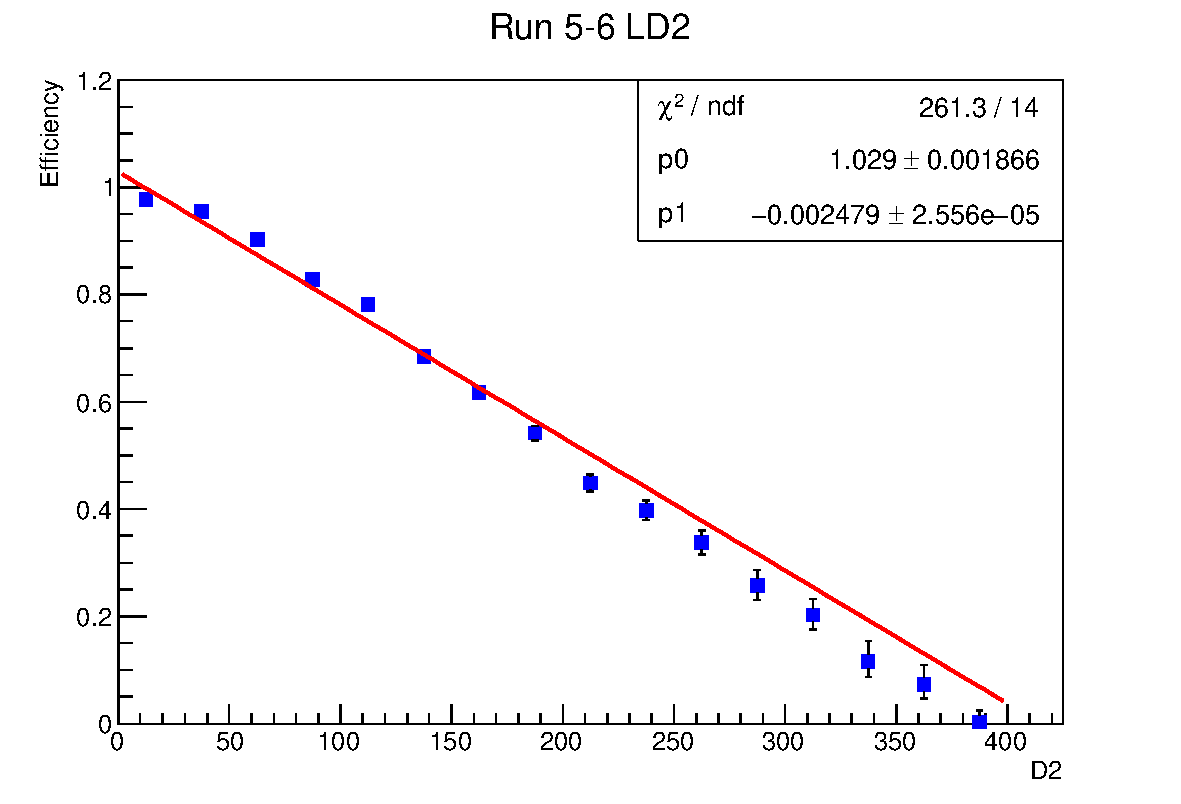
\includegraphics[width=0.5\linewidth]{run5-6_Drell-Yan_LD2}
	\caption{The reconstruction efficiency plotted as a function of station 2 occupancy, calculated using
		Run~5 \ce{LD_2} Drell-Yan MCs.
		The efficiency is calculated by taking the ratio of messy MC events over clean MC events in each
		occupancy bin. Standard cuts were applied to both numerator and denominator
		(except the occupancy cut on clean MC).
	}
	\label{fig:tracking efficiency}
\end{figure}

This tracking efficiency can also depend on the dimuon kinematics. This can be caused
by the noise hits being more localized in some area of the detector, which can map to
different kinematic phase space. To study this effect, we repeat the study with different
Monte Carlo, and the extract efficiency is tabulated in \cref{tab:track_eff_DY,tab:track_eff_jpsi,tab:track_eff_psip}. The extracted efficiency
are consistent with each other within uncertainties.

\begin{table}
	\centering
	\caption{The extracted tracking efficiency from Drell-Yan Monte Carlo}
	\label{tab:track_eff_DY}
	\begin{tabular}{|l|l|l|l|l|l|}
\hline
Run                  & target & Intercept & Error on intercept & slope    & Error on slope \\ \hline
\multirow{2}{*}{2-3} & \ce{LH_2}    & 0.9887    & 0.0053             & -0.00251 & 0.000021       \\ \cline{2-6} 
                     & \ce{LD_2}    & 1.0072    & 0.0056             & -0.00257 & 0.000021       \\ \hline
\multirow{2}{*}{5-6} & \ce{LH_2}    & 1.0218    & 0.002              & -0.00243 & 0.000027       \\ \cline{2-6} 
                     & \ce{LD_2}    & 1.029     & 0.0019             & -0.00248 & 0.000026       \\ \hline
\end{tabular}

\end{table}
\begin{table}
	\centering
	\caption{The extracted tracking efficiency from $J/\psi$  Monte Carlo}
	\label{tab:track_eff_jpsi}
	\begin{tabular}{|l|l|l|l|l|l|}
	\hline
	Run                  & target    & intercept              & slope                   \\ \hline
	\multirow{2}{*}{2-3} & \ce{LH_2} & $1.0544    \pm 0.0143$ & $-0.00268 \pm 0.000021$ \\ \cline{2-4}
	                     & \ce{LD_2} & $1.0453    \pm 0.0152$ & $-0.00269 \pm 0.000045$ \\ \hline
	\multirow{2}{*}{5-6} & \ce{LH_2} & $1.025     \pm 0.0044$ & $-0.00245 \pm 0.000071$ \\ \cline{2-4}
	                     & \ce{LD_2} & $1.0214    \pm 0.0045$ & $-0.00245 \pm 0.000067$ \\ \hline
\end{tabular}

\end{table}
\begin{table}
	\centering
	\caption{The extracted tracking efficiency from $\psi'$ Monte Carlo}
	\label{tab:track_eff_psip}
	\begin{tabular}{|l|l|l|l|l|l|}
	\hline
	Run                  & target    & Intercept                & slope                   \\ \hline
	\multirow{2}{*}{2-3} & \ce{LH_2} & $1.035     \pm 0.0117$   & $-0.00265 \pm 0.000044$ \\ \cline{2-4}
	                     & \ce{LD_2} & $1.028     \pm 0.01146$  & $-0.00265 \pm 0.000035$ \\ \hline
	\multirow{2}{*}{5-6} & \ce{LH_2} & $1.024     \pm 0.003647$ & $-0.00259 \pm 0.000059$ \\ \cline{2-4}
	                     & \ce{LD_2} & $1.022     \pm 0.00442$  & $-0.00268 \pm 0.000059$ \\ \hline
\end{tabular}

\end{table}

Once the tracking efficiency is obtained from the Monte Carlo, the efficiency correction ($\epsilon_{recon.Eff}$)
is calculated, which is defined as the average of the inverse of tracking efficiency in each
kinematic bin. This correction is calculated separately for each target, as a denser target
will produce more hits in the detector. This is shown in \cref{fig:target_D2}.

\begin{figure}[h!]
	\centering
	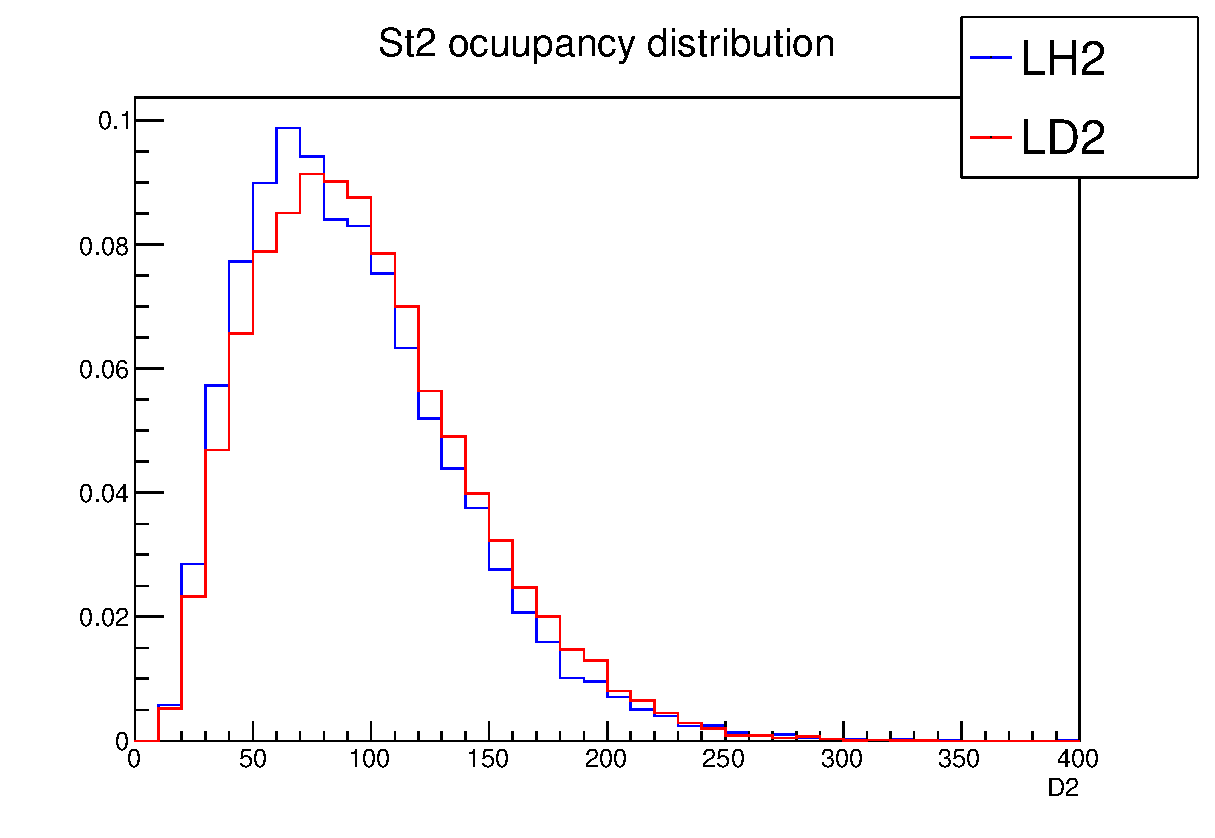
\includegraphics[width=0.5\linewidth]{run5-6_DY_D2}
	\caption{The St.~2 occupancy profile for \ce{LH_2} and \ce{LD_2} for run 5-6 after event selection. Both histograms are normalized to unit area.
	}
	\label{fig:target_D2}
\end{figure}


\section{Absolute \texorpdfstring{$J/\psi$}{J/psi} Cross Section Extraction}
The charmonium yield is extracted from the data using the mass fit method.
Separate mass fits are done independently for each kinematic bin. After obtaining
the yield, various corrections are needed, including the tracking efficiency, target
contamination correction and acceptance correction.
\subsection{Target Contamination}
\label{subsec:contamination}
For a pure target, the cross section can be obtained from the yield using the following
\begin{equation}
	B\sigma = \frac{Y A}{T N_A P X \epsilon},
\end{equation}
where $Y$ is the extracted yield, $A$ is the atomic mass of the target,
$T$ is the thickness of the target, $N_A$ is the Avogadro’s number,
$P$ is the proton on target, $\epsilon$ is the acceptance and efficiency correction,
and $X$ is the beam attenuation factor given by
\begin{equation}
	X=\frac{\lambda}{L\rho} \left[1-\exp\left(-\frac{L\rho}{\lambda}\right)\right],
\end{equation}
where $\lambda$ is the interaction length, $L$ and $\rho$ are the length and density
of the target. And $B$ is the branching ratio for decaying into a dimuon pair, which is need
 to obtain the production cross section. The branching ratios used are taken from Ref.~\cite{workman2022}.
\begin{equation}
	B\left(J/\psi\to\mu^+\mu-\right)=5.961\times 10^{-2},\quad B\left(\psi'\to\mu^+\mu-\right)=8\times 10^{-3}.
\end{equation}

The liquid targets are held in a flask \SI{50.8}{\cm} long and \SI{7.62}{\cm} in diameter
and can contain \SI{2.2}{\l} of liquid. The liquid Hydrogen used is \SI{99.999}{\percent}
pure. On the other hand, the Deuterium used came from two sources:
\begin{itemize}
	\item \SI{95.8\pm0.2}{\percent} pure deuterium that was used for bubble chamber experiments
	      at Fermilab, with contamination in the form of \ce{HD}.
	\item \SI{99.99}{\percent} pure commercial deuterium which is used in later part of the experiment.
\end{itemize}
\begin{table}[h!]
	\centering
	\caption{Summary of \ce{LD_2} contamination, taken from Ref.~\cite{don-4993}}
	\label{table:LD2_contamination}
	\begin{tabular}{|l|ll|l|l|}
		\hline
		Sample no. & \multicolumn{2}{l|}{\ce{D_2} bottle no.} & Sample date & description                                                                                                                          \\ \hline
		1          & \multicolumn{1}{l|}{Fermilab}            & 53          & 4/12/18     & \SI{95.6}{\percent} \ce{D}, \SI{4.4}{\percent} \ce{H}; \SI{92}{\percent}  \ce{D_2}, \SI{8}{\percent} \ce{HD} gases     \\
		2          & \multicolumn{1}{l|}{Fermilab}            & 113         & 4/12/18     & \SI{96}{\percent} \ce{D}, \SI{4}{\percent} \ce{H}; \SI{93}{\percent}  \ce{D_2}, \SI{7}{\percent} \ce{HD} gases         \\
		3          & \multicolumn{1}{l|}{Fermilab}            & 53          & 4/12/18     & just air; gas must have leaked                                                                                         \\
		4          & \multicolumn{1}{l|}{Matheson}            & 127         & 4/12/18     & about half air; remaining \SI{99.1}{\percent} \ce{D}, \SI{0.3}{\percent} \ce{H}                                        \\
		5          & \multicolumn{1}{l|}{Matheson}            & 2           & 4/12/18     & sample for test purposes; not analyzed                                                                                 \\
		6          & \multicolumn{1}{l|}{Matheson}            &             & 7/28/16     & more than half air; remaining \SI{99.3}{\percent} \ce{D}, \SI{0.7}{\percent} \ce{H}                                    \\
		7          & \multicolumn{1}{l|}{Matheson}            &             & 5/28/17     & \SI{99.8}{\percent} \ce{D}, \SI{0.2}{\percent} \ce{H}; \SI{99.6}{\percent}  \ce{D_2}, \SI{0.4}{\percent} \ce{HD} gases \\ \hline
	\end{tabular}
\end{table}
Therefore, care is needed to account for the contribution from the hydrogen contamination in deuterium
target data. The result of the mass spectroscopy of the deuterium gas \cite{don-4993} is
summarized in \cref{table:LD2_contamination}. Based on this analysis, it is concluded the Fermilab
deuterium contains \SI{91.6}{\percent} \ce{D_2} and \SI{8.4}{\percent} \ce{HD} by moles. \pdfcomment{need to check this sentence.}

The yield from the contaminated deuterium can be expressed as
\begin{equation}
	Y_{\mathrm{cont.~\ce{LD_2}}} = N_A P_D X_D \epsilon_D \left( T_D^D \sigma_{pd}/A_D + T^D_H \sigma_{pp}/A_H   \right).
\end{equation}
Here $T_D^D$ and $T^D_H$ are the thickness of deuterium and hydrogen in the deuterium target.
$A_H$ and $A_D$ are the atomic mass of hydrogen and deuterium.
The subscript $D$ denotes these deuterium target specific quantities.

In order to extract the $T_D^D$ and $T^D_H$ from the mole fraction listed in \cref{table:LD2_contamination},
we first note that the volume of a \ce{HD} molecule is about \num{1.094} times the volume of a \ce{D_2}
molecule. Therefore the effective volume of molecules in the target is
\begin{equation}
	\begin{split}
		V_{\mathrm{eff.}}&=\frac{N_{\ce{HD}} V_{\ce{HD}} + N_{\ce{D_2}} V_{\ce{D_2}}}{N_{\text{tot.}}}\\
		&=V_{D_2} \left[ C \frac{V_{\ce{HD}}}{V_{\ce{D_2}}} + (1-C) \right]\\
		&=V_{D_2} f,
	\end{split}
\end{equation}
where $C=N_{\ce{HD}}/N_{\ce{D_2}}$ and $f=\left[ C V_{\ce{HD}}/V_{\ce{D_2}} + (1-C) \right]$ with the
volume ratio $V_{\ce{HD}}/V_{\ce{D_2}}=1.094$.
The total number of molecules per area is
\begin{equation}
	\begin{split}
		\frac{N_{\mathrm{tot.}}}{\mathrm{Area}} &= \frac{L}{V_{\mathrm{eff.}}}\\
		&= \frac{L}{V_{\ce{D_2}}f}=\frac{L\rho_{\ce{D_2}}}{2A_Df}.
	\end{split}
\end{equation}
The thickness of D (in \unit{\g\per\cm\squared}) in the target cell is
\begin{equation}
	\begin{split}
		T_D^D &= \frac{N_D A_D}{\mathrm{Area}} = A_D\frac{N_{\mathrm{tot.}}}{\mathrm{Area}} \left[ 2(1-C) + C \right]\\
		&=A_D \frac{L\rho_{\ce{D_2}}}{2A_Df}(2-C)\\
		&=\frac{L\rho_{\ce{D_2}}}{f}(1-C/2).
	\end{split}
\end{equation}
The thickness of H (in \unit{\g\per\cm\squared}) in the target cell is
\begin{equation}
	\begin{split}
		T^D_H &= \frac{N_H A_H}{\mathrm{Area}} = A_H\frac{N_{\mathrm{tot.}}}{\mathrm{Area}}C\\
		&=\frac{L\rho_{\ce{D_2}}}{f}\frac{A_H}{A_D}\frac{C}{2}.
	\end{split}
	\label{eq:TDH}
\end{equation}
To determine the density of the deuterium target, the vent pressure is measured and is compared
with NIST database to obtained the expected density for pure deuterium ($\rho_{\ce{D_2}}$) \cite{density-1453}.
For contaminated deuterium, the effective density is
\begin{equation}
	\begin{split}
		\rho_{\mathrm{eff.}} &= \frac{1}{L} (T_D^H + T_D^D)\\
		&=\frac{\rho_{\ce{D_2}}}{f} \left[ \frac{A_H}{A_D}\frac{C}{2}+(1-C/2) \right],
	\end{split}
\end{equation}
and the effective interaction length is
\begin{equation}
	\begin{split}
		\frac{1}{\lambda_{\mathrm{eff.}}} &= \frac{1}{L\rho_{\mathrm{eff.}}} \left[\frac{T_D^H}{\lambda_H} +\frac{T_D^D}{\lambda_D}\right]\\
		&=\left[\frac{A_H}{A_D}\frac{C}{2\lambda_H} + \frac{1-C/2}{\lambda_D}\right]\left( \frac{A_H}{A_D}\frac{C}{2} +(1-C/2)\right)^{-1}.
	\end{split}
\end{equation}

Note that in previous studies and publications, including Ref.~\cite{dove2021,dove2023},
the ratio of atomic mass is missing in \cref{eq:TDH}.
This results in a roughly \SI{2}{\percent} difference in the cross section ratio
that will be discussed in \cref{M-subsubsec:contamination_result}.

Including the contamination correction, the deuterium cross section is
\begin{equation}
	\sigma_{pd} = \frac{Y_{\ce{LD_2}} A_D}{T_D^D N_A P_D X_{\mathrm{eff.}} \epsilon_D} - \frac{T^D_H}{T_D^D} \frac{A_D}{A_H} \sigma_{pp},
\end{equation}
where the hydrogen cross section is
\begin{equation}
	\sigma_{pp} = \frac{Y_{\ce{LH_2}} A_H}{T_H^H N_A P_D X_{H} \epsilon_H}.
\end{equation}
And the cross section ratio is given by
\begin{equation}
	\frac{\sigma_{pd}}{2\sigma_{pp}} = \frac{Y_{\ce{LD_2}}}{2Y_{\ce{LH_2}}}\frac{A_D}{A_H}\frac{T_H^H P_H X_{H} \epsilon_H}{T_D^D P_D X_{\mathrm{eff.}} \epsilon_D} - \frac{T^D_H}{2T_D^D} \frac{A_D}{A_H}.
\end{equation}

The switch to commercial pure deuterium gas happened during Roadset 67 data taking. Therefore,
an average contamination, weighted by the proton on target, is used for the entire dataset.
The average contamination for entire roadset 57 -70 data is determined to be $C=\SI{5.95}{\percent}$.
Therefore the effective values for target contamination for this dataset are
\begin{equation}
	\begin{split}
		T_D^H &= \SI{0.1230}{\g\per\cm\squared}, \\
		T_D^D &= \SI{8.009}{\g\per\cm\squared},\\
		\rho_{\mathrm{eff.}} & = \SI{0.1601}{\g\per\cm\squared},\\
		\lambda_{\mathrm{eff.}} &= \SI{71.39}{\g\per\cm\squared},\\
		\lambda_{\mathrm{eff.}}/\rho_{\mathrm{eff.}} &= \SI{446.0}{\cm},\\
		X_{\mathrm{eff.}} &= 0.9451.
	\end{split}
\end{equation}
For later runs where commercial pure deuterium is used,
\begin{equation}
	\begin{split}
		T_D^H &= \SI{0.}{\g\per\cm\squared}, \\
		T_D^D &= \SI{8.30072}{\g\per\cm\squared},\\
		\rho_{\mathrm{eff.}} & = \rho_{\ce{D_2}} = \SI{0.1634}{\g\per\cm\squared},\\
		\lambda_{\mathrm{eff.}} &=  \lambda_{\ce{D_2}} =\SI{71.80}{\g\per\cm\squared},\\
		\lambda_{\mathrm{eff.}}/\rho_{\mathrm{eff.}} &= \SI{439.4}{\cm},\\
		X_{\mathrm{eff.}} &= 0.9444.
	\end{split}
\end{equation}
And since there is no contamination in the \ce{LH_2} target
\begin{equation}
	\begin{split}
		\rho_{H_2} &= \SI{0.0708}{\g\per\cm\cubed},\\
		T_H^H &= L\rho_{\ce{H_2}} = \SI{3.597}{\g\per\cm\squared},\\
		\lambda_H/\rho_{\ce{H_2}} &= \SI{734.5}{\cm},\\
		X_H &=0.9662.
	\end{split}
\end{equation}


\subsection{Acceptance Calculation}
The acceptance is obtained by comparing the results of clean Monte Carlo analysis with thrown distribution,
and is defined as follows
\begin{equation}
	\epsilon_{acc.}\left(\Omega\right)=\mathrm{Acceptance}\left(\Omega\right)= \frac{N_{accept}\left(\Omega\right)}{N_{thrown}\left(\Omega\right)},
\end{equation}
where $N_{accept}\left(\Omega\right)$ is the number of accepted events in a given kinematic bin $\Omega$
by analyzing the clean Monte Carlo , with the same dimuon selection
as the data, while $N_{thrown}$ is the total number of generated Monte Carlo events in the same kinematic bin.
The clean Monte Carlo is used in the acceptance calculation with the explicit intent to separate out the
rate dependent effects.

The histogram in the numerator is filled using the reconstructed kinematics, whereas
the thrown histogram in the denominator is filled using the thrown kinematics. This accounts for
the first order effect of bin migration, caused by the spectrometer resolution.

%Since our histograms are weighted histograms, the uncertainty is calculated using the following
\pdfcomment{verify the uncertainty calculation here}

The calculated acceptance for $J/\psi$ and $\psi'$ are shown in \cref{fig:jpsi_acceptance,fig:psip_acceptance}.
The $\psi'$ acceptance is also larger then the $J/\psi$, primarily due to the
trigger matrix being optimized for the high mass dimuons. The acceptance is also larger at forward $x_F$,
as would be expected for a forward spectrometer.
At the later runs the trigger requirements have been relaxed to allow for more low mass events.
This is also reflected in the figures.
\begin{figure}[h!]
	\centering
	\begin{subfigure}{0.45\linewidth}
		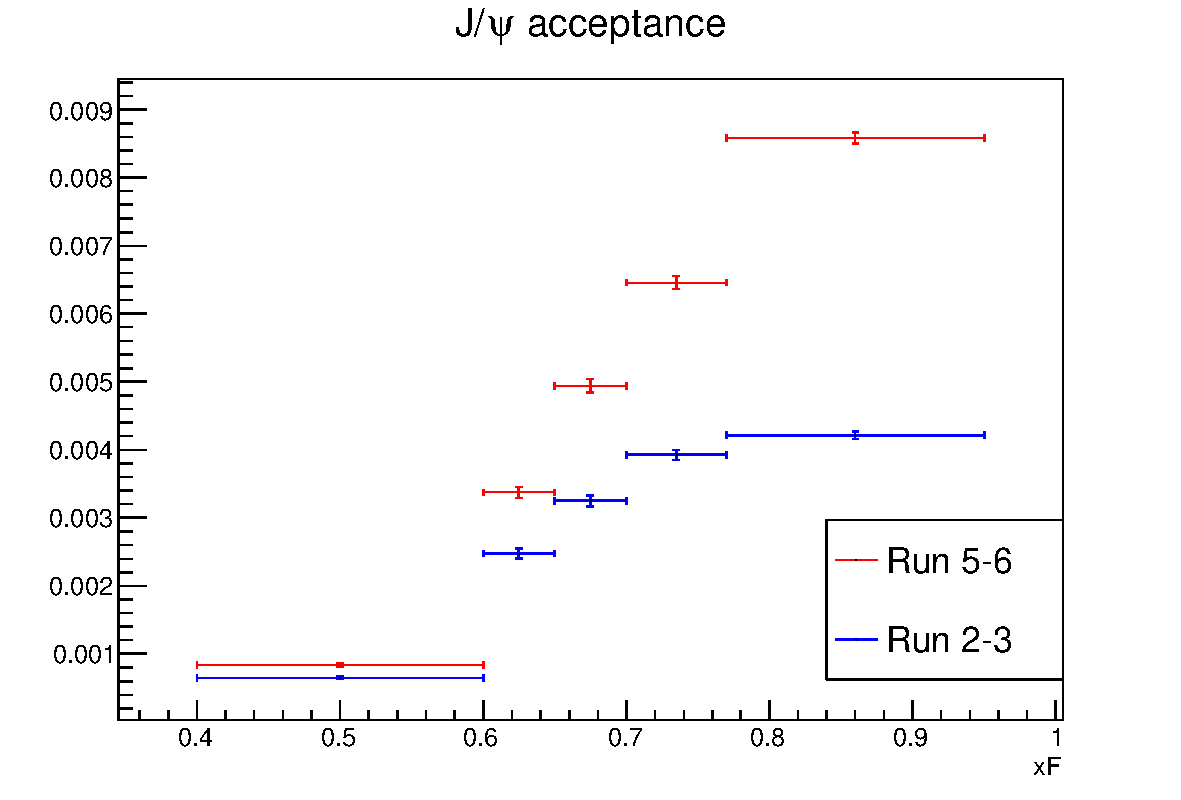
\includegraphics[width=0.9\linewidth]{acceptance/jPsi_acceptance_xF}
		\caption{$x_F$ acceptance}
	\end{subfigure}
	\begin{subfigure}{0.45\linewidth}
		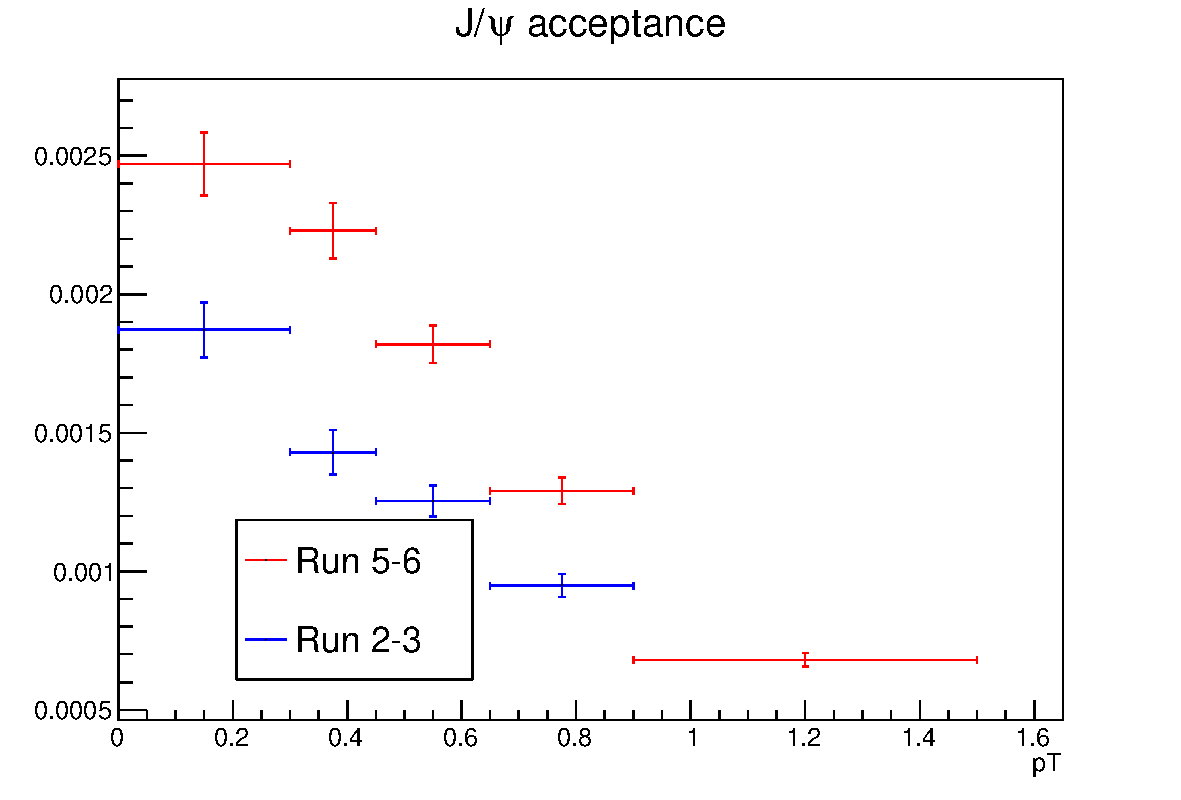
\includegraphics[width=0.9\linewidth]{acceptance/jPsi_acceptance_pT}
		\caption{$p_T$ acceptance}
	\end{subfigure}
	\caption{Spectrometer acceptance for the $J/\psi$}
	\label{fig:jpsi_acceptance}
\end{figure}
\begin{figure}[h!]
	\centering
	\begin{subfigure}{0.45\linewidth}
		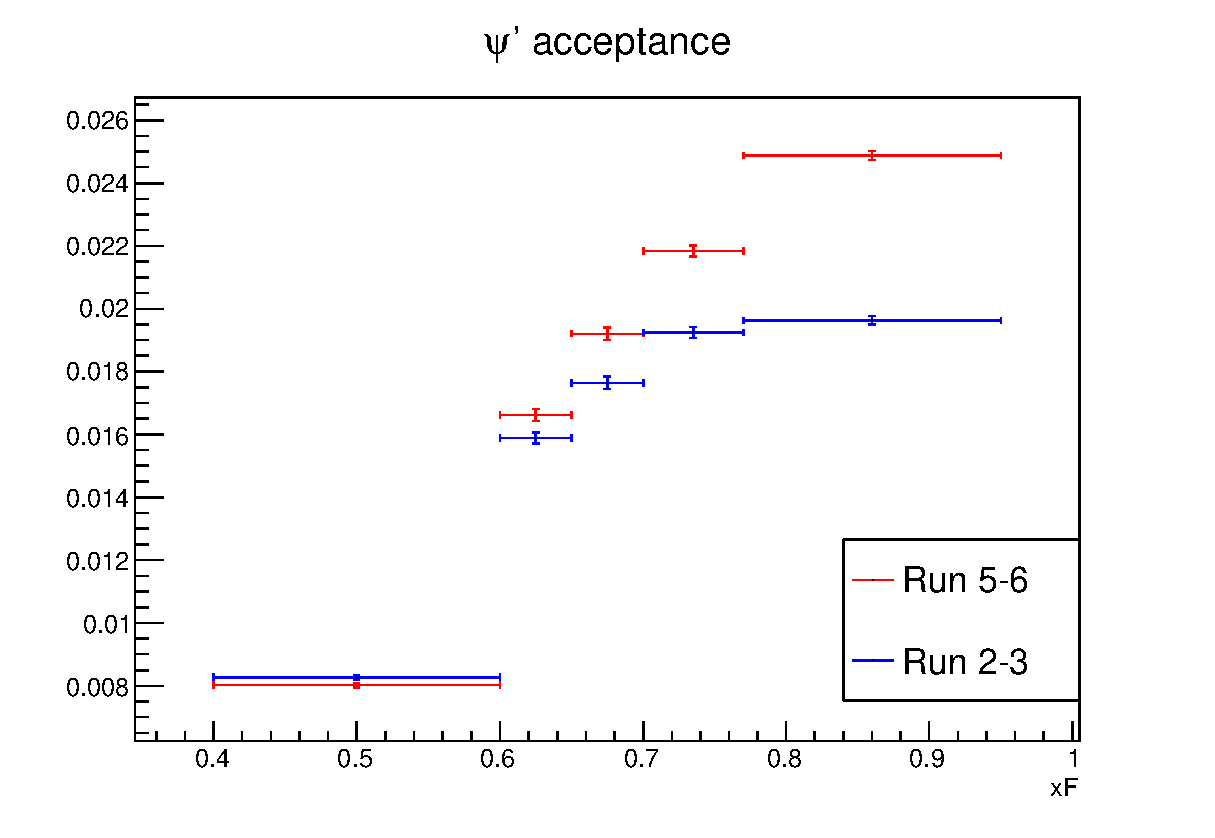
\includegraphics[width=0.9\linewidth]{acceptance/psip_acceptance_xF}
		\caption{$x_F$ acceptance}
	\end{subfigure}
	\begin{subfigure}{0.45\linewidth}
		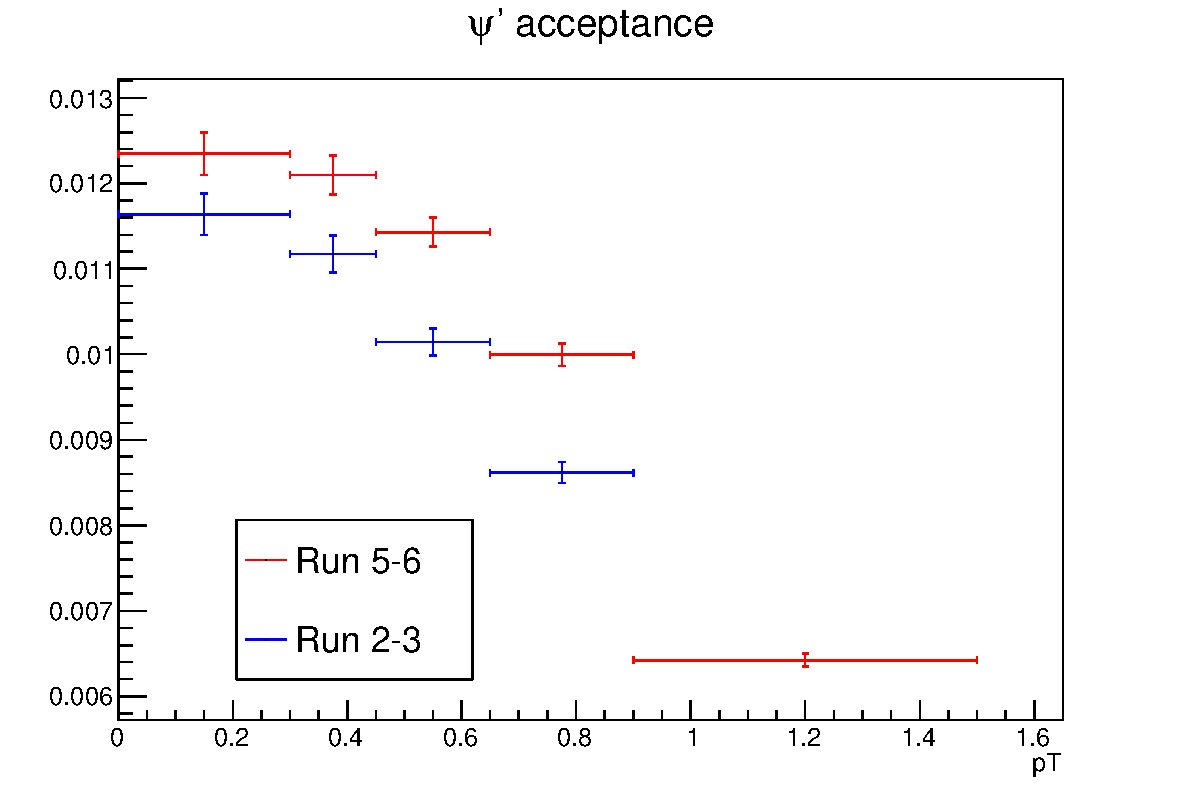
\includegraphics[width=0.9\linewidth]{acceptance/psip_acceptance_pT}
		\caption{$p_T$ acceptance}
	\end{subfigure}
	\caption{Spectrometer acceptance for the $\psi'$}
	\label{fig:psip_acceptance}
\end{figure}
\section{Comparison of data with Monte Carlo}

\subsection{\texorpdfstring{$P_T$}{P\_T} distribution}
A first order $P_T$ reweighting for the Drell-Yan MC is performed in this analysis. The acceptance is first
calculated using the original Monte Carlo data. While the $P_T$ is known be incorrect,
the extracted acceptance as a function for $P_T$ should not depend on the input
distribution. The $P_T$ distribution from the empty flask subtracted data
is plotted in 3 $x_F$ bins. A \SI{4.5}{\GeV} mass cut is applied to remove contribution for the
resonances. The acceptance corrected distributions are fitted to \cref{eq:kaplan} to
extract the $p1$ parameter in each bin. The extracted $p1$ is shown in \cref{fig:p1_xF_DY},
and it is also fitted to a first order polynomial. The $p1(x_F)$ extracted is used in calculating
the $P_T$-reweighting. And the $p_1\left(x_F\right)$ is given by
\begin{equation}
	\begin{split}
		p_1 = 2.411 - 0.7658 \abs{x_F} \quad \text{for \ce{LH_2}}\\
		p_1 = 2.394 - 0.7576 \abs{x_F} \quad \text{for \ce{LD_2}}
	\end{split}
\end{equation}

\begin{figure}[h!]
	\centering
	\begin{subfigure}{0.45\linewidth}
		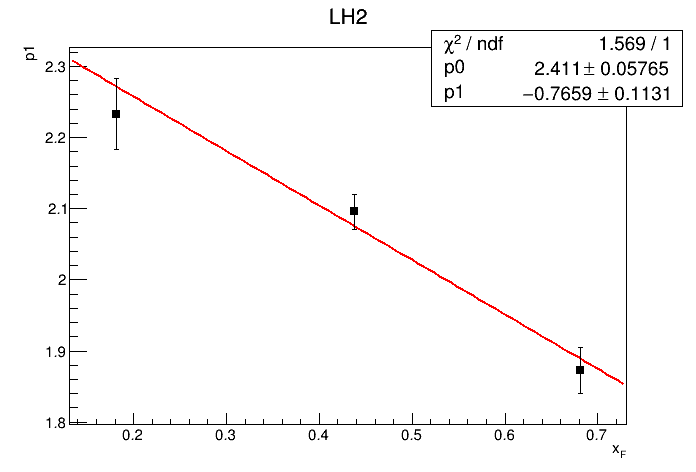
\includegraphics[width=\linewidth]{pT_reweight/LH2_DY_p1}
	\end{subfigure}
	\begin{subfigure}{0.45\linewidth}
		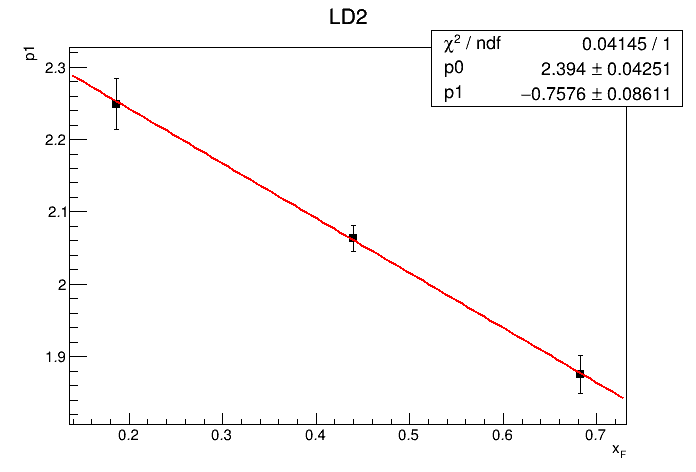
\includegraphics[width=\linewidth]{pT_reweight/LD2_DY_p1}
	\end{subfigure}
	\caption{The extracted $p1$ from \ce{LH_2}(right) and \ce{LD_2} data as a function
		$x_F$ and fitted to a first order polynomial.}
	\label{fig:p1_xF_DY}
\end{figure}
As seen in \cref{fig:p1_xF_DY}, the $p_1$ (and therefore $\expval{P_T}$) decreases as $x_F$ increases.
As $x_F$ increases, more of the available energy are taken by the dimuon longitudinal momentum,
therefore the $P_T$ distribution should be narrower.
This is also consistent to previous studies in Ref.~\cite{prasad2020} and the maximum $P_T$ discussed in
\cref{subsec:messyMC}.

For the charmonium decays, the $P_T$ distribution is extracted in a iterative process, and the $p1$
parameters used are $1.735$ for $J/\psi$ and $1.620$ for $\psi'$, and are consistent with the result in
\cref{M-tab:kaplan_result}.

\section{Intensity Extrapolation}
\label{sec:extrapolation}
An independent method for extracting the Drell-Yan cross section ratio, known as intensity extrapolation method, 
is first studied by J.~Dove~\cite{dove2020} and A.~Tadepalli~\cite{tadepalli2019}, 
and it is used in Ref.~\cite{dove2021}.
The assumption behind this method is that the accidental background and physics events
would have different intensity dependence. The number of observed physics
events, in the absence of any spectrometer effects, should be linearly proportional to the beam
intensity. On the contrary, the two muons in the accidental background are typically coming from
two separate interactions, and therefore it is expected to be proportional to the intensity squared.
By taking the ratio of the $(p+p)$ and $(p+d)$ dimuon event rates,
other rate dependent effects would also be canceled out at zero intensity.

The procedure for this method is summarized here. A mass cut at \SI{4.5}{\GeV} is applied to
remove the charmonium decays, leaving only the Drell-Yan dimuons and the accidental background.
Cuts are also applied to exclude region close to the boundaries of the acceptance.
Then the background originated from the interaction with the instruments is estimated by using
the empty flask data normalized by the integrated beam intensity, and is subtracted from the
$p+p$ and $p+d$ data. Third, the $(p+d)/2(p+p)$ ratios are formed by empty flask subtracted
dimuon data, normalized by the raw proton ratios. The ratio is calculated as a function of the
instantaneous beam intensity measured by the BIM. The ratio is then fitted with the following function
\begin{equation}
	R_i \left(I\right) = p_{0i} + p_1 I + p_2 I^2,
	\label{eq:common_pol2}
\end{equation}
where the parameter $p_1$ and $p_2$ are common to all bins, and the intercept $p_{0i}$ gives
the value of the cross section ratio in each $x_T$ bins. Other fit functions are also used
to study the fit function dependence.

\begin{figure}
	\centering
	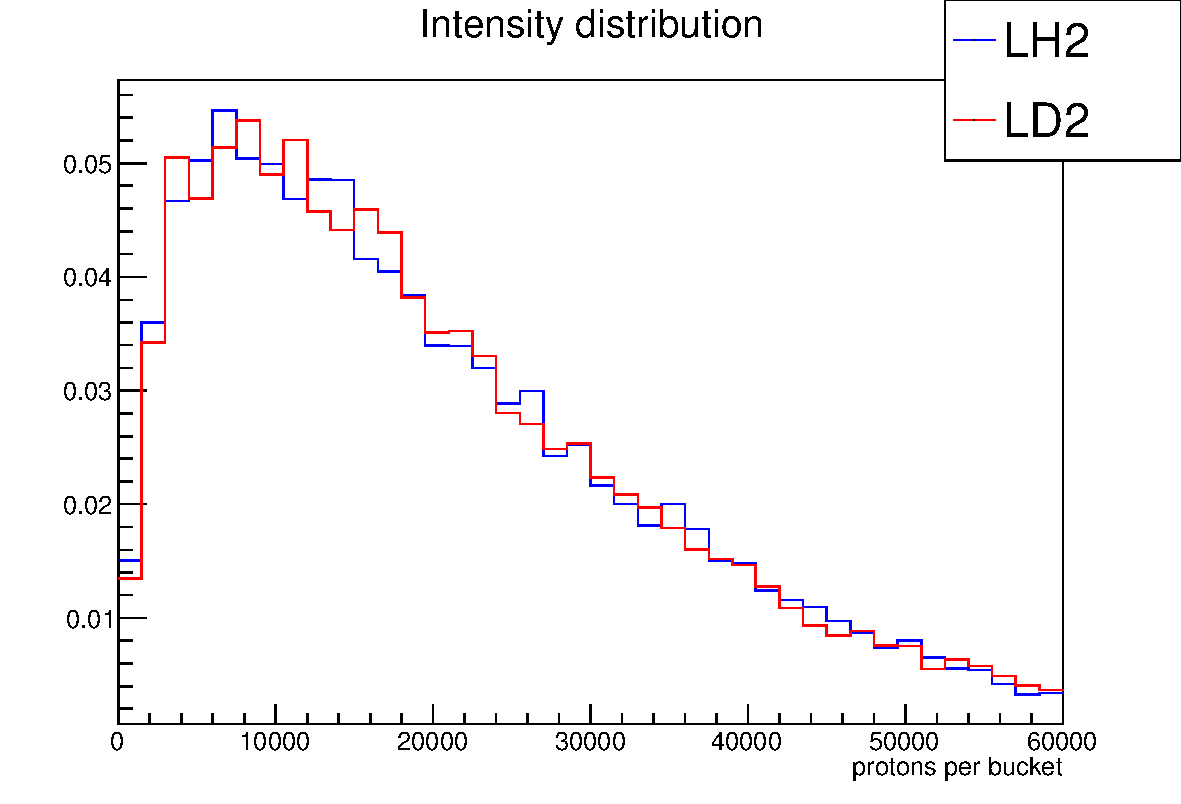
\includegraphics[width=0.6\linewidth]{run5-6_DY_tInt}
	\caption{The intensity distribution of the reconstructed from Run 5-6 after applying the event selection.
		The distributions are normalized to unit area.}
	\label{fig:tInt_distribution}
\end{figure}

\pdfcomment{explain choice of raw proton}

While this method allows for extractions of the Drell-Yan cross section ratio without relying
heavily on simulation, this method cannot be used in the charmonium studies.
Both Drell-Yan process and charmonium production would have the same linear intensity dependence,
hence this method is not able to distinguish the different physics processes, and therefore could
not be used in the charmonium studies. Moreover, only the cross section ratio could be obtained in
this method, as the absolute yield and value of rate dependency correction will be needed in
absolute cross section studies, and cannot be obtained from the intensity extrapolation method.

\section{Systematic uncertainties}
For the Drell-Yan cross section ratios studies, the intensity extrapolation method and mass fit
method involve different assumptions and therefore different sources of systematic uncertainties.
\paragraph{Proton beam normalization}
The beam normalization uncertainty is present in all studies presented here.
As described in \cref{sec:beam_norm}, the number of protons are measured by the BIM, which is
calibrated against a SEM monitor. The SEM monitor is further calibrated by studying the activation of
an irradiated high purity copper foil. A copper foil is placed in the beam line near the monitor,
causing the production of \ce{^{24}Na}. The \ce{^{24}Na} then decay into \ce{^{24}Mg} through $\beta$
decay. The number of  \ce{^{24}Na} nuclei is deduced by counting the number \SI{1369}{\keV} photons
produced. Using the \SI{3.56}{\milli\barn} production cross section for \ce{^{24}Na} in natural
copper  by \SI{120}{\GeV} protons, the number of incident protons can be deduced. The estimated
random uncertainty in the counting and extraction of \SI{1369}{\keV} peak is $\sim 1-2\%$.
An additional \SI{8}{\percent} systematic uncertainty in the production cross section of \ce{^{24}Na}
is also included \cite{docdb-457,docdb-7708}.
A total of \SI{10}{\percent} beam normalization uncertainty is assigned to absolute cross
section studies, whereas a \SI{2}{\percent} relative normalization uncertainty is assigned to ratios between
targets. This \SI{2}{\percent} relative normalization uncertainty is also included in the empty flask
subtraction.

\paragraph{Choice of fit function}
This is specific to the cross section ratio studies using intensity extrapolation method.
To estimate the effect of the choice of fit function, different fit functions were examined.
For example, we can allow the $p_1$ and $p_2$ parameters in \cref{eq:common_pol2} to have kinematic
dependence
\begin{equation}
	R_i \left(I\right) = p_{0i} + \left[p_{10}+p_{11}x_i\right] I + \left[p_{20}+p_{21}x_i\right] I^2,
\end{equation}
where $x_i$ is the kinematic average in each bin. The difference of the result obtained with different fit
functions is included in the systematic uncertainty.

\paragraph{Mixed background}
This is specific to studies using mass fit method. Different mixing methods have been proposed in SeaQuest.
The mixed sample from the two methods described in \cref{sec:mixing} are used. The difference between
the two analyses is included in the systematic uncertainty.

\paragraph{Acceptance simulation}
This is a major systematics in the absolute cross section studies, particularly when using
Run 2-3 data.
During Run 2-3, multiple trigger road sets were used. However, due to the limited statistics in each
data taking period, it is not possible to analyze each subset separately. Therefore these datasets
are combined into one. While the difference in trigger road sets has little effect on the acceptance
for the high mass Drell-Yan dimuon \cite{jdove-8168}, the impact on the $J/\psi$ acceptance is much
larger \cite{chleung-9643}.

During later runs, only one trigger road set (roadset 78) was used, hence this is no
longer an issue.


\section{Drell-Yan NLO calculation}
\label{sec:DYNNLO}
The next-to-leading order (NLO) calculation is done using a parton level Monte
Carlo program, named DYNNLO, written by the INFN group~\cite{catani2009,catani2007}. This program
is originally written to compute cross section for vector boson
production from $p+p$ and $p+\bar{p}$ collisions. It was later modified, in
collaboration with W.C.~Chang and S.~Prasad, to perform $p+n$ calculation
by utilizing charge symmetry. The $p+d$ interaction can be computed by summing up
the $p+p$ and $p+n$ calculation, assuming no nuclear corrections. For heavier nuclear
targets, nuclear PDFs can also be used. It is also modified to calculate $x_F$, $x_1$ and $x_2$
using the same definition as SeaQuest as discussed in \cref{subsec:def_kinematic}.

The PDF sets used in this study are CT18~\cite{hou2021} and NNPDF4.0~\cite{ball2022a}.
And they are accessed through the LHAPDF library~\cite{buckley2015}. It should be noted
that the CT18 PDF set is published before the SeaQuest result, whereas NNPDF4.0
incorporate the SeaQuest measurements~\cite{dove2021} in the global fit.

The uncertainty band for calculations using CT18 PDFs are calculated using the hessian methods.
Given a central PDF member $S_0$ and $2N_{\mathrm{par}}$ eigenvector PDF member $S^\pm_i$ ($i=1,\dots,N_{\mathrm{par}}$),
where $N_{\mathrm{par}}$ is the number of parameters. The central value $F_0$ and the uncertainty $\sigma^\pm_F$
on a PDF-dependent quantity are given by:
\begin{equation}
	\begin{split}
		F_0 &= F(S_0),\quad F_i^\pm=F(S_i^\pm) \\
		\sigma^+_F &= \sqrt{\sum_{i=1}^{N_{\mathrm{par}}} \left[\max\left(F_i^+ - F_0, F_0 - F^-_i,0\right)\right]^2 }\\
		\sigma^-_F &= \sqrt{\sum_{i=1}^{N_{\mathrm{par}}} \left[\max\left(F_0 - F^+_i, F_i^- - F_0,0\right)\right]^2 }
	\end{split}
\end{equation}

Whereas the uncertainty for NNPDF4.0 is calculated using the replicas method. Given $N_{\mathrm{rep}}$ replica
PDF members $S^k$, the central value and the uncertainty is given by the mean and standard deviation
\begin{equation}
	\begin{split}
		F_0&=\expval{F}=\frac{1}{N_{\mathrm{rep}}}\sum_{i=1}^{N_{\mathrm{rep}}}F\left(S^k\right)\\
		\sigma_F&= \sqrt{\frac{1}{N_{\mathrm{rep}}-1}\sum_{i=1}^{N_{\mathrm{rep}}}\left[F\left(S^k\right)-F_0\right]^2}
	\end{split}
\end{equation}

It should also be noted that CT18 reports the \SI{90}{\percent} confidence level by default, whereas NNPDF4.0
would report the \SI{68}{\percent} confidence level.

The DYNNLO calculation requires two energy scales, the factorization and renormalization scales,
as introduced in \cref{M-subsec:scaling_violation}. Since the DYNNLO code was designed to calculate
vector boson production cross section at the LHC, the scale is originally chosen to be the W boson mass (\SI{80.385}{\GeV}).
The SeaQuest data covers the mass of \SI{4.5}{\GeV} to \SI{8.8}{\GeV} for the Drell-Yan
process. The original chosen scale is certainly too high for fixed target experiments.
It is recommended by the authors to pick a scale of the order of the dimuon mass.
Instead of using a fixed scale, we chose to turn on dynamic scale,
where both factorization and renormalization scales would be dynamically set to the dimuon mass at
each iteration.  The difference between using a fixed scale and dynamic scales is shown in \cref{fig:DY_scale}.
The overall difference is small, as the chosen fixed scale is within the dimuon mass range of interest.
The effect is more significant when the difference between the chosen fixed scale and the dimuon mass
becomes larger.
\begin{figure}[h!]
	\centering
	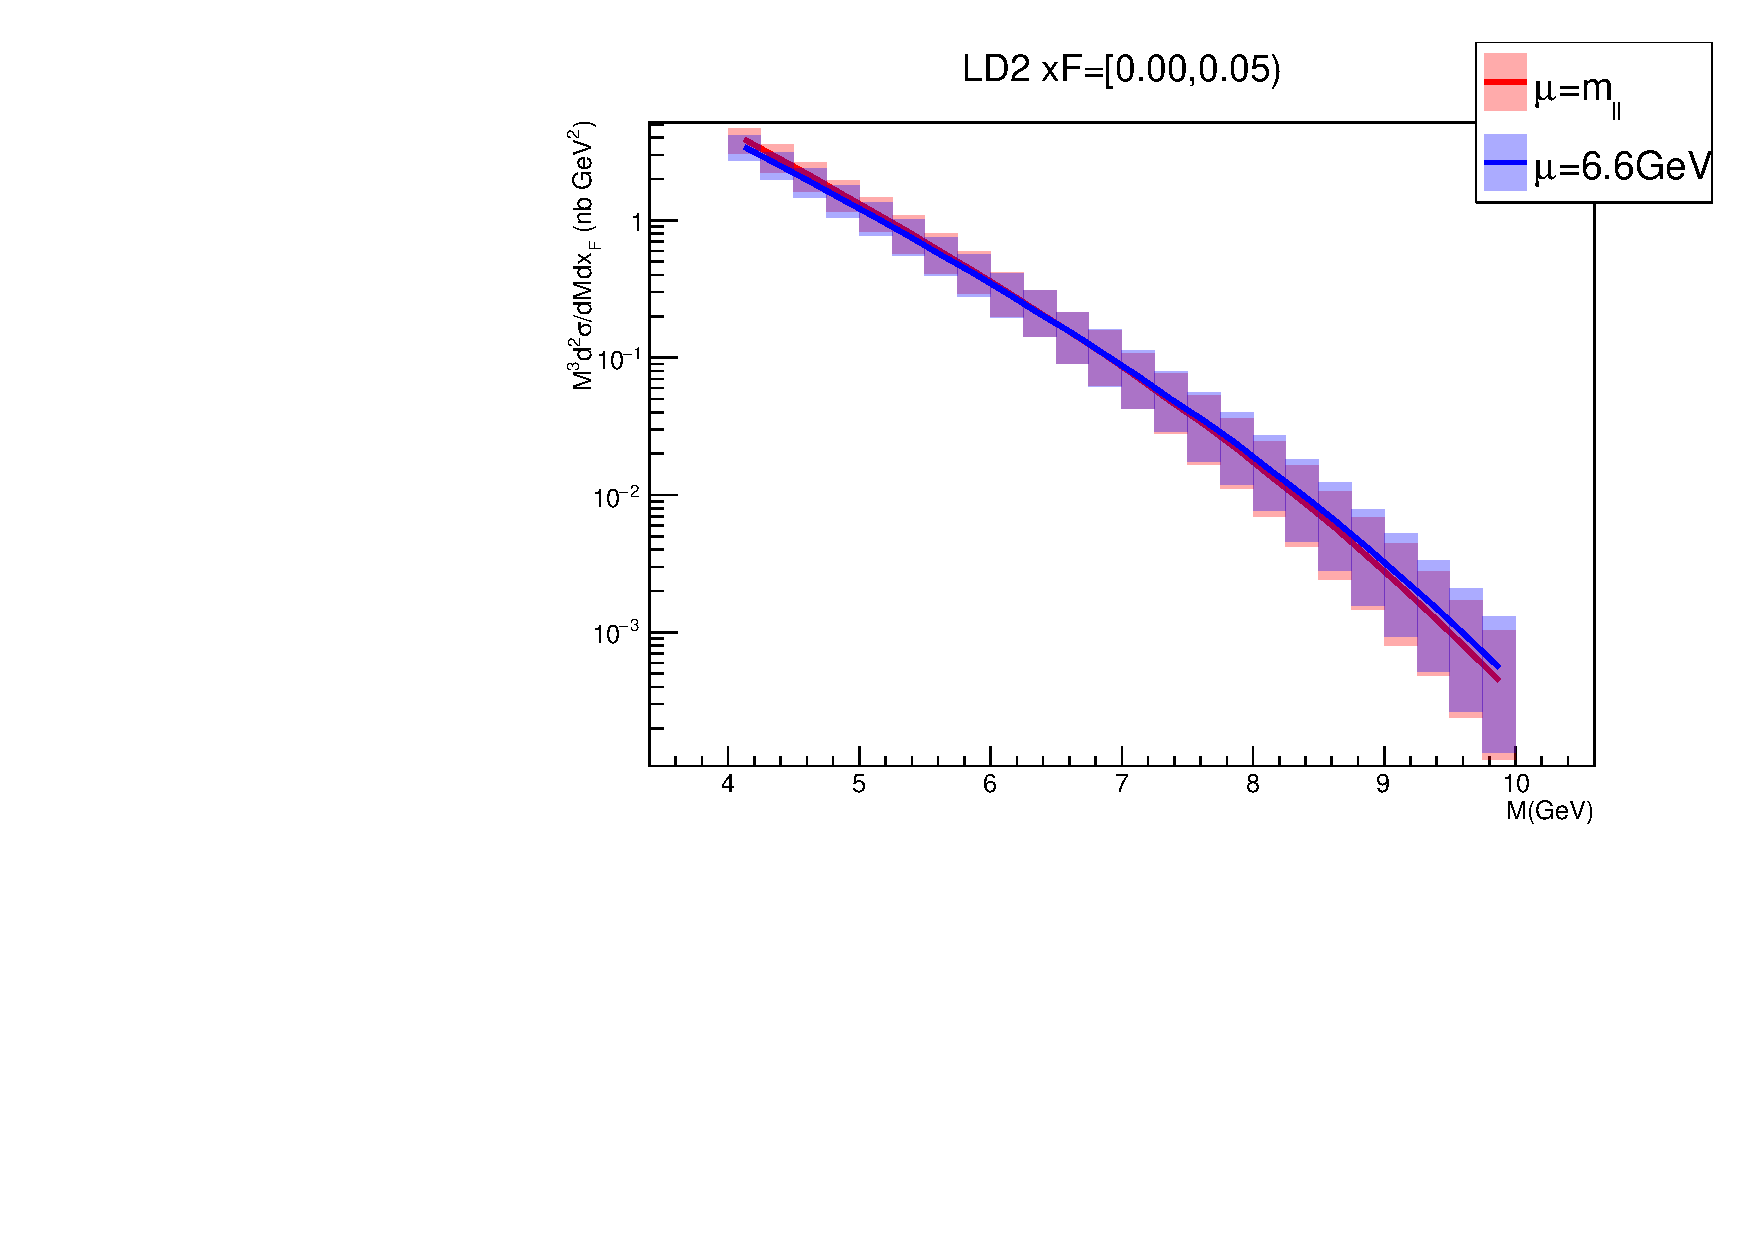
\includegraphics[width=0.6\linewidth]{scale/dy_cs0_d.pdf}
	\caption{The calculated Drell-Yan cross section using a fixed scale compared with using dynamic scales.
		The uncertainty bands denotes the \SI{90}{\percent} confident level from CT18NLO PDF.
	}
	\label{fig:DY_scale}
\end{figure}




\ifSubfilesClassLoaded{ \printbibliography[heading=bibintoc,title={References}]}{}
\end{document}
